%Version 3.1 December 2024
%%%%%%%%%%%%%%%%%%%%%%%%%%%%%%%%%%%%%%%%%%%%%%%%%%%%%%%%%%%%%%%%%%%%%%
%%                                                                 %%
%% Please do not use \input{...} to include other tex files.       %%
%% Submit your LaTeX manuscript as one .tex document.              %%
%%                                                                 %%
%%%%%%%%%%%%%%%%%%%%%%%%%%%%%%%%%%%%%%%%%%%%%%%%%%%%%%%%%%%%%%%%%%%%%

\documentclass[referee,lineno,pdflatex,sn-vancouver-num]{sn-jnl}

%%%% Standard Packages
\usepackage{graphicx}%
\usepackage{multirow}%
\usepackage{amsmath,amssymb,amsfonts}%
\usepackage{amsthm}%
\usepackage{mathrsfs}%
\usepackage[title]{appendix}%
\usepackage{xcolor}%
\usepackage{textcomp}%
\usepackage{manyfoot}%
\usepackage{booktabs}%
\usepackage{algorithm}%
\usepackage{algorithmicx}%
\usepackage{algpseudocode}%
\usepackage{tikz}%
\usetikzlibrary{arrows.meta,positioning,calc,decorations.pathreplacing}%
\usepackage{pgfplots}%
\pgfplotsset{compat=1.18}%

\begin{document}

\title[PRIMED: Joint Loss Estimation for Multi-Reader Imaging Data]{PRIMED: Joint Loss Estimation with Selective Penalization for Multi-Reader Imaging Data with Binary Outcomes}

%%=============================================================%%
%% Author information
%%=============================================================%%

\author[1]{\fnm{Yonghan} \sur{Kwon}}\email{yonghankwon0@yuhs.ac}

\author*[1]{\fnm{Kyunghwa} \sur{Han}}\email{khhan@yuhs.ac}

\affil*[1]{\orgdiv{Department of Radiology, Research Institute of Radiological Science, and Center for Clinical Imaging Data Science}, \orgname{Yonsei University College of Medicine}, \orgaddress{\city{Seoul}, \country{Republic of Korea}}}

%%================================%%
%% Structured abstract for BMC   %%
%%================================%%

\abstract{\textbf{Background:} When multiple readers independently assess the same medical image, their interpretations frequently disagree. Conventional approaches treat this inter-reader variability as nuisance to be eliminated, yet it may carry predictive information. Existing methods for incorporating variability focus on single longitudinal biomarkers and do not address the high-dimensional, multivariate setting of multi-reader imaging data where variable selection is required.

\textbf{Methods:} We propose PRIMED (Penalized Regularization for Integrated Multi-path Estimation with Dispersion), a joint loss framework that integrates three information channels: consensus (mean reader score), disagreement (standard deviation across readers), and the structural relationship between them. A dispersion model captures how each feature's consensus determines its disagreement, and only the residual disagreement (the component not explained by consensus) enters the outcome model. A group LASSO penalty on the outcome coefficients performs variable selection, while dispersion parameters remain unpenalized. Performance is evaluated through simulation studies and two applications: a multi-center, multi-reader MRI study of 149 rectal cancer patients (14 features, 5 readers) and the LIDC-IDRI lung nodule dataset (107 radiomics features, 1,390 nodules, 3--4 readers).

\textbf{Results:} In simulations across multiple settings (varying signal-to-noise ratio, noise levels, and dimensionality up to 100 features), PRIMED achieves the highest F1 score and AUC in the majority of settings, with advantages driven primarily by higher positive predictive value. Variable selection stability, measured by the Jaccard index, is highest for PRIMED at all dimensionalities (e.g., 0.248 vs.\ 0.217 and 0.218 at 100 features). In the rectal cancer application, PRIMED selects features missed by competing methods. In the LIDC-IDRI application, PRIMED achieves comparable prediction (10-fold cross-validated AUC 0.900) with substantially higher selection stability (Jaccard 0.798 vs.\ 0.688 and 0.560).

\textbf{Conclusions:} PRIMED provides a principled framework for exploiting inter-reader disagreement in multi-reader imaging studies. By jointly modeling the consensus--disagreement relationship and using residual disagreement as a predictor, it achieves superior variable selection with consistent stability across replications, while maintaining competitive prediction performance. Validation on two distinct imaging modalities (MRI and CT) and scales (14 to 107 features) confirms these advantages generalize across clinical settings.}

\keywords{Multi-reader imaging, Variable selection, Group LASSO, Inter-reader disagreement, Consensus--disagreement framework, Rectal cancer, Radiomics, LIDC-IDRI, Lung nodule}

\maketitle

%%===================================================================
\section{Background}\label{sec:background}
%%===================================================================

When multiple readers independently assess the same medical image, their interpretations frequently disagree.
This inter-reader variability is ubiquitous across imaging modalities and clinical tasks: radiologists differ in contouring tumor boundaries on MRI \cite{BeetsTan2018,MERCURY2006}, in scoring subjective features such as fibrosis or diffusion restriction, and in delineating nodule margins on CT \cite{Armato2011}.
The conventional approach treats such disagreement as nuisance to be eliminated.
Reliability coefficients such as the intraclass correlation coefficient \cite{Shrout1979} and kappa \cite{Fleiss1971} quantify it, summary strategies (averaging, majority voting) remove it, and measurement error methods such as regression calibration and SIMEX \cite{Carroll2006,Cook1994} correct for the attenuation it induces.
All of these strategies discard variability rather than use it.

Yet a growing body of evidence suggests that variability itself can carry predictive information.
In other areas of medicine, variability has been recognized as a predictor in its own right: visit-to-visit blood pressure variability predicts stroke and cardiovascular events independently of mean blood pressure \cite{Rothwell2010,Diaz2014}.
Joint models \cite{Gao2022,Yu2024} and mixed-effects location-scale models \cite{Hedeker2008} have been developed to incorporate within-subject variability into outcome prediction.
These approaches, however, focus on a single biomarker measured longitudinally and do not address the high-dimensional, multivariate setting of multi-reader imaging, where $K$ features are assessed simultaneously and variable selection is required.
This gap is particularly acute in modern radiomics, where hundreds of quantitative features are extracted from segmentation masks that differ across readers, producing a rich but unexploited source of inter-reader disagreement information.

This raises a fundamental question: when multiple readers assess the same image, should their disagreement simply be eliminated, or can it be harnessed for prediction?

A natural starting point is to treat both the consensus (mean of reader scores, $\bar{X}_k$) and the disagreement (standard deviation, $S_k$) as predictors in a penalized regression, a perspective we term the consensus--disagreement (CD) framework.
This approach, however, faces an important obstacle: $\bar{X}_k$ and $S_k$ are generally not independent.
On bounded ordinal scales, a boundary effect forces disagreement toward zero when the consensus is near the extremes \cite{Taylor1961,Taylor2019}.
Beyond this mechanical constraint, reader-specific factors such as differential confidence at different score levels produce feature-specific consensus--disagreement relationships whose direction and strength vary across features.
If $S_k$ is entered alongside $\bar{X}_k$ without accounting for this dependence, a feature can appear to carry disagreement signal simply because its disagreement tracks its consensus level, not because residual disagreement predicts the outcome.
In high-dimensional settings with many inactive features, this conflation inflates false positives and destabilizes variable selection.

A straightforward implementation of the CD framework is to apply a group penalty \cite{Yuan2006} to each feature's consensus--disagreement pair, or to penalize only the consensus mean via the LASSO \cite{Tibshirani1996}.
Either approach treats the two summaries as independent inputs and ignores the structural relationship described above.

To address this gap, we propose PRIMED (Penalized Regularization for Integrated Multi-path Estimation with Dispersion), a joint loss framework that integrates three information channels: consensus, disagreement, and the structural relationship between them.
The key idea is to fit a dispersion model that captures how each feature's consensus determines its disagreement, and to feed only the \emph{residual} disagreement, the component not explained by consensus, into the outcome model.
Because the outcome model depends on these residuals, the dispersion parameters $\alpha_k$ receive gradient contributions from both the dispersion and outcome losses, yielding genuinely joint estimation rather than a two-stage procedure.
A group penalty is applied only to the outcome coefficients $(\beta_k, \gamma_k)$, so that variable selection reflects outcome relevance alone.
We demonstrate the framework through simulation studies and two real-data applications: a multi-reader MRI study of rectal cancer ($K = 14$, $m = 5$ readers) and a high-dimensional radiomics study of lung nodule malignancy ($K = 107$, $m = 3$--$4$ readers).

%%===================================================================
\section{Methods}\label{sec:methods}
%%===================================================================

%%-------------------------------------------------------------------
\subsection{Data structure}\label{sec:data}
%%-------------------------------------------------------------------

Consider $n$ subjects, $K$ imaging features, and $m$ readers.
Let $x_{ijk}$ denote the score assigned by reader $j$ ($j = 1,\dots,m$) to subject $i$ ($i = 1,\dots,n$) on feature $k$ ($k = 1,\dots,K$).
For each subject--feature pair, define the consensus (sample mean across readers) and the disagreement (sample standard deviation across readers); alternative choices of these summary statistics for different measurement scales are discussed in Appendix~\ref{secA1}:
\[
  \bar X_{ik} = \frac{1}{m}\sum_{j=1}^m x_{ijk}, \qquad
  S_{ik} = \left[\frac{1}{m-1}\sum_{j=1}^m (x_{ijk} - \bar X_{ik})^2\right]^{1/2}.
\]
If the number of readers varies across subjects (e.g., due to missing evaluations or, as in the LIDC-IDRI application, varying numbers of annotators per nodule), $m$ is replaced by the subject-specific count $m_i$ in the definitions above.
Let $Y_i \in \{0,1\}$ denote the binary outcome for subject $i$.
The observed data thus consist of the consensus matrix $\bar X \in \mathbb{R}^{n \times K}$, the disagreement matrix $S \in \mathbb{R}^{n \times K}$, and the outcome vector $Y \in \{0,1\}^n$.

%%-------------------------------------------------------------------
\subsection{Consensus--disagreement framework}\label{sec:cd_framework}
%%-------------------------------------------------------------------

Rather than discarding $S$, we treat both $\bar X$ and $S$ as potential predictors of $Y$, a perspective we call the consensus--disagreement (CD) framework.
Two baseline strategies arise naturally within this framework.
The first, which we term the \emph{CD group LASSO} (CD~GL), regresses $Y$ on the full set $(\bar X_1, S_1, \dots, \bar X_K, S_K)$ with a group LASSO penalty \cite{Yuan2006} that links each $(\bar X_k, S_k)$ pair, so that consensus and disagreement for a given feature are selected or dropped together.
The second, the \emph{consensus LASSO} (C~LASSO), regresses $Y$ on $(\bar X_1, \dots, \bar X_K)$ with an $\ell_1$ penalty \cite{Tibshirani1996}, using only the consensus and ignoring the disagreement channel entirely.

Both methods enter $\bar X_k$ and $S_k$ as independent inputs.
As noted in Section~\ref{sec:background}, however, $\bar X_k$ and $S_k$ are generally correlated, and this structural relationship varies in direction and strength across features.
Including $S_k$ alongside $\bar X_k$ without accounting for their dependence conflates the direct contribution of disagreement with the part that merely reflects the consensus level, potentially distorting coefficient estimates and variable selection.
PRIMED addresses this limitation by explicitly modeling the consensus--disagreement relationship and decomposing disagreement into a structurally explained component and a residual, as described next.

%%-------------------------------------------------------------------
\subsection{Joint loss function}\label{sec:joint_loss}
%%-------------------------------------------------------------------

The PRIMED loss comprises two components (a dispersion loss and an outcome loss), each normalized by its respective null baseline.
Figure~\ref{fig:path} illustrates the overall structure: the dispersion model (top) links consensus to disagreement, and the outcome model (bottom) uses both consensus and residual disagreement as predictors.

Because the consensus and disagreement of a feature are generally correlated, entering both into an outcome model without accounting for this dependence confounds their individual contributions.
The dispersion loss captures this relationship explicitly: for each feature $k$, a linear regression links consensus to disagreement:
$S_{ik} = \alpha_{0k} + \alpha_k \bar X_{ik} + \varepsilon_{ik}$,
where $\alpha_{0k}$ is the feature-specific intercept, $\alpha_k$ is the slope quantifying how the consensus level affects disagreement, and $\varepsilon_{ik}$ is the residual error.
The squared-error loss and its null baseline (intercept-only model, i.e., $\alpha_k = 0$ for all $k$) are
\[
  \mathcal{L}_{\mathrm{disp}} = \frac{1}{2n}\sum_{k=1}^K \sum_{i=1}^n (S_{ik} - \alpha_{0k} - \alpha_k \bar X_{ik})^2,
  \qquad
  \mathcal{L}_{\mathrm{disp}}^0 = \frac{1}{2}\sum_{k=1}^K \widehat{\mathrm{Var}}(S_k).
\]

The dispersion model defines, for each subject--feature pair, the residual disagreement
\[
  \tilde S_{ik} = S_{ik} - \alpha_{0k} - \alpha_k \bar X_{ik},
\]
i.e., the part of reader disagreement that is not explained by the consensus level.
This residual is the quantity used in the outcome model, ensuring that $\gamma_k$ captures the effect of disagreement \emph{beyond} what is structurally linked to the consensus.

The outcome model is a logistic regression of $Y_i$ on both the consensus and the residual disagreement predictors.
Let $\beta_0$ denote the intercept, $\beta_k$ the coefficient for the consensus predictor of feature $k$, and $\gamma_k$ the coefficient for the residual disagreement predictor of feature $k$.
The predicted probability for subject $i$ is
$p_i = \mathrm{logit}^{-1}\!\bigl(\beta_0 + \sum_{k=1}^K \beta_k \bar X_{ik} + \sum_{k=1}^K \gamma_k \tilde S_{ik}\bigr)$.
If $\alpha_k$ were estimated by OLS on the dispersion model alone, $\tilde S_k$ would be exactly sample-orthogonal to $\bar X_k$ by construction, and $\beta_k$ and $\gamma_k$ would capture non-overlapping components of the linear predictor.
In the joint estimation, the coupling gradient (Section~\ref{sec:optimization}) can shift $\alpha_k$ away from the OLS solution when $\gamma_k \neq 0$, so the exact orthogonality is approximate rather than exact; it holds precisely for features with $\gamma_k = 0$.

The negative log-likelihood and its null baseline (intercept-only model, predicting the marginal proportion $\bar Y = n^{-1}\sum_i Y_i$) are
\[
  \mathcal{L}_{\mathrm{out}} = -\frac{1}{n}\sum_{i=1}^n \bigl[Y_i \log p_i + (1-Y_i)\log(1-p_i)\bigr],
  \qquad
  \mathcal{L}_{\mathrm{out}}^0 = -\bigl[\bar Y \log \bar Y + (1-\bar Y)\log(1-\bar Y)\bigr].
\]

Because the outcome loss depends on the residual disagreement $\tilde S_{ik}$, which is itself a function of $\alpha$, the joint loss couples $\alpha$ to both components:
\begin{equation}\label{eq:joint_loss}
  \mathcal{L}(\boldsymbol{\alpha}, \boldsymbol{\beta}, \boldsymbol{\gamma}) = \frac{\mathcal{L}_{\mathrm{disp}}(\boldsymbol{\alpha})}{\mathcal{L}_{\mathrm{disp}}^0}
              + \frac{\mathcal{L}_{\mathrm{out}}(\boldsymbol{\alpha}, \boldsymbol{\beta}, \boldsymbol{\gamma})}{\mathcal{L}_{\mathrm{out}}^0}.
\end{equation}
Each component is normalized by its null value so that both terms start at 1.0 under the null model, eliminating the need for a weighting hyperparameter.
The dependence of $\mathcal{L}_{\mathrm{out}}$ on $\boldsymbol{\alpha}$ through $\tilde S_{ik}$ is the mechanism that achieves genuinely joint estimation of the dispersion and outcome parameters.

%%-------------------------------------------------------------------
\subsection{Penalty structure}\label{sec:penalty}
%%-------------------------------------------------------------------

Let $\boldsymbol{\alpha} = (\alpha_1,\dots,\alpha_K)^T$, $\boldsymbol{\beta} = (\beta_1,\dots,\beta_K)^T$, and $\boldsymbol{\gamma} = (\gamma_1,\dots,\gamma_K)^T$ collect the slope coefficients across all features, and let $\lambda > 0$ denote the regularization parameter controlling sparsity.
The penalized objective is
\begin{equation}\label{eq:objective}
  \min_{\boldsymbol{\alpha}, \boldsymbol{\beta}, \boldsymbol{\gamma}} \;\;
  \mathcal{L}(\boldsymbol{\alpha}, \boldsymbol{\beta}, \boldsymbol{\gamma})
  \;+\; \lambda \sum_{k=1}^K \sqrt{\beta_k^2 + \gamma_k^2}.
\end{equation}
The penalty is a group LASSO norm applied to the outcome coefficients $(\beta_k, \gamma_k)$ for each feature $k$.
The group structure ensures that each feature is evaluated holistically (considering both its consensus signal ($\beta_k$) and its residual disagreement signal ($\gamma_k$)), rather than allowing one channel to be selected in isolation, which could lead to the inclusion of features with a spurious consensus or disagreement effect.
Since each group consistently contains two coefficients, the standard $\sqrt{p_g}$ weight reduces to $\sqrt{2}$ for all groups. This constant factor is absorbed into the proximal threshold (see Section~\ref{sec:optimization}), so no group-specific weighting is needed.

The intercepts $\alpha_{0k}$ and $\beta_0$ are unpenalized, as is standard.
Crucially, the dispersion slopes $\alpha_k$ are also unpenalized: they are updated by gradient descent without penalty-induced shrinkage.
Although $\alpha_k$ receives no penalty, it is \emph{not} estimated in a separate stage: because $\mathcal{L}_{\mathrm{out}}$ depends on $\alpha_k$ through $\tilde S_{ik}$, the gradient of the outcome loss with respect to $\alpha_k$ provides an additional update signal (see Section~\ref{sec:optimization}).
This selective penalization ensures that the consensus--disagreement relationship is estimated without penalty-induced bias regardless of outcome relevance, while variable selection is driven solely by the outcome coefficients $(\beta_k, \gamma_k)$.

All predictors ($\bar X_k$ and $S_k$) are standardized to zero mean and unit variance within the training set prior to penalization, ensuring that the group LASSO penalty is applied on a common scale across features with different units.

Feature $k$ is selected if $\hat\beta_k \neq 0$ or $\hat\gamma_k \neq 0$.

%%-------------------------------------------------------------------
\subsection{Optimization}\label{sec:optimization}
%%-------------------------------------------------------------------

We minimize~\eqref{eq:objective} via proximal gradient descent (Algorithm~\ref{alg:primed}).
Let $\eta > 0$ denote the step size (learning rate).
At each iteration, all parameters receive a gradient step.
The dispersion parameters $(\alpha_{0k}, \alpha_k)$ receive gradients from \emph{two} sources: the dispersion loss $\mathcal{L}_{\mathrm{disp}}$ and, because $\tilde S_{ik} = S_{ik} - \alpha_{0k} - \alpha_k \bar X_{ik}$ enters the outcome model, the outcome loss $\mathcal{L}_{\mathrm{out}}$.
The coupling gradient for $\alpha_k$ from the outcome loss is
\[
  \frac{\partial (\mathcal{L}_{\mathrm{out}}/\mathcal{L}_{\mathrm{out}}^0)}{\partial \alpha_k}
  = -\frac{\gamma_k}{n\,\mathcal{L}_{\mathrm{out}}^0} \sum_{i=1}^n (p_i - Y_i)\,\bar X_{ik},
\]
which arises because $\partial \tilde S_{ik}/\partial \alpha_k = -\bar X_{ik}$.
This gradient vanishes when $\gamma_k = 0$ (i.e., when feature $k$ is not selected), so only outcome-relevant features couple the two losses.
More precisely, at any stationary point the gradient of $\mathcal{L}$ with respect to $\alpha_k$ satisfies
\begin{equation}\label{eq:stationary_alpha}
  \underbrace{\frac{1}{n\,\mathcal{L}_{\mathrm{disp}}^0}\sum_{i=1}^n \tilde S_{ik}\,\bar X_{ik}}_{\text{dispersion gradient}}
  \;=\;
  \underbrace{-\frac{\gamma_k}{n\,\mathcal{L}_{\mathrm{out}}^0}\sum_{i=1}^n (p_i - Y_i)\,\bar X_{ik}}_{\text{coupling gradient}}.
\end{equation}
Because the joint objective is non-convex (see below), \eqref{eq:stationary_alpha} characterizes any stationary point reached by the algorithm, not a unique global solution.
At such a point, when $\gamma_k = 0$ the right-hand side vanishes, so $\sum_i \tilde S_{ik}\,\bar X_{ik} = 0$: the residual $\tilde S_k$ is sample-orthogonal to $\bar X_k$, and $\hat\alpha_k$ coincides with the ordinary least squares estimate.
When $\gamma_k \neq 0$, $\hat\alpha_k$ departs from the OLS solution; the coupling gradient shifts $\alpha_k$ in a direction that reduces the joint loss, producing a purposeful bias in the dispersion model that benefits outcome prediction.
The outcome intercept $\beta_0$ is updated by standard gradient descent.
The outcome coefficients $(\beta_k, \gamma_k)$ then receive a group-wise proximal (soft-thresholding) step:
\[
  (\beta_k, \gamma_k) \leftarrow
  \begin{cases}
    \displaystyle \Bigl(1 - \frac{\eta\lambda\sqrt{2}}{\|(\tilde\beta_k, \tilde\gamma_k)\|_2}\Bigr)
    (\tilde\beta_k, \tilde\gamma_k),
    & \text{if } \|(\tilde\beta_k, \tilde\gamma_k)\|_2 > \eta\lambda\sqrt{2}, \\[6pt]
    (0,0), & \text{otherwise},
  \end{cases}
\]
where $(\tilde\beta_k, \tilde\gamma_k)$ denotes the post-gradient values.
This proximal operator is the key mechanism that sets entire $(\beta_k, \gamma_k)$ pairs exactly to zero, producing group-wise sparsity.
The dispersion coefficients $\alpha_k$ are never shrunk, ensuring that the consensus--disagreement relationship is estimated without penalty-induced bias regardless of outcome relevance.

Convergence is declared when the relative change in parameters falls below a tolerance $\epsilon = 10^{-6}$, or after a maximum of $10{,}000$ iterations.
In practice, the step size $\eta = 0.005$ provides stable convergence across all settings examined.

We note that the joint objective~\eqref{eq:objective} is non-convex in $(\boldsymbol{\alpha}, \boldsymbol{\beta}, \boldsymbol{\gamma})$ jointly, because $\mathcal{L}_{\mathrm{out}}$ contains the bilinear product $\gamma_k \alpha_k$ through the residual $\tilde S_{ik}$.
The objective is convex in $\boldsymbol{\alpha}$ with $(\boldsymbol{\beta}, \boldsymbol{\gamma})$ fixed, and convex in $(\boldsymbol{\beta}, \boldsymbol{\gamma})$ with $\boldsymbol{\alpha}$ fixed, so the proximal gradient algorithm converges to a stationary point but not necessarily a global minimum.
In our experiments, convergence was robust to initialization and we did not observe sensitivity to local minima.

A practical concern with non-convex objectives is that the regularization path may be non-monotone: decreasing $\lambda$ could, in principle, cause previously selected features to drop out, because the change in $\hat\alpha_k$ alters $\tilde S_{ik}$ and thereby reshapes the loss landscape.
In convex group LASSO, path monotonicity (the number of selected features increases as $\lambda$ decreases) is mathematically guaranteed; no such guarantee exists for PRIMED.
To assess this empirically, we traced the full regularization path on the LIDC-IDRI dataset ($K = 107$), evaluating 50 log-spaced $\lambda$ values from $\lambda_{\max}$ (0 features selected) to $\lambda_{\max}/1000$ (all 107 features selected), each from a cold start (zero initialization).
The path was strictly monotone: the number of selected features increased or remained constant at every step, with zero violations across 49 transitions.
Figure~\ref{fig:path_mono} visualizes the result: the number of selected features increases smoothly from 0 (at $\lambda_{\max}$) to 107 (at $\lambda_{\max}/1000$), with no reversals.
This suggests that, despite the theoretical non-convexity, the bilinear coupling between $\alpha_k$ and $\gamma_k$ does not disrupt path regularity in practice, likely because the dispersion model is well identified for most features and the coupling gradient produces only small perturbations around the OLS solution for $\alpha_k$.


\begin{figure}[h]
\centering
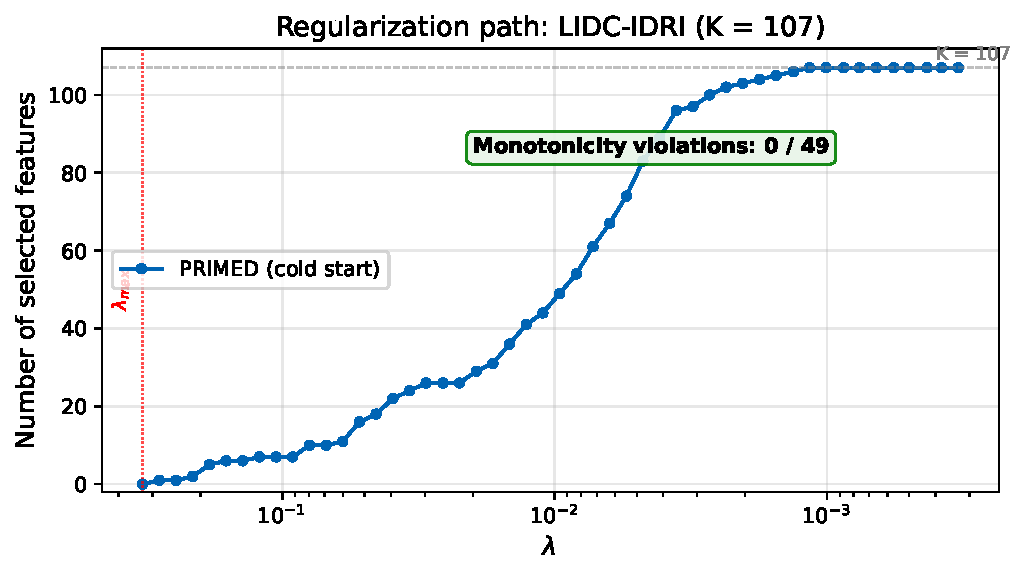
\includegraphics[width=0.75\textwidth]{fig_path_monotonicity.pdf}
\caption{Regularization path for PRIMED on the LIDC-IDRI dataset. Each point represents an independent fit from zero initialization (cold start) at a given $\lambda$ with $K = 107$ features.
The number of selected features increases monotonically as $\lambda$ decreases, with zero violations across 49 transitions.
Despite the non-convexity of the joint objective, the path exhibits the same monotone behavior as convex group LASSO.}\label{fig:path_mono}
\end{figure}


%%-------------------------------------------------------------------
\subsection{Coefficient interpretation}\label{sec:properties}
%%-------------------------------------------------------------------

Substituting $\tilde S_{ik} = S_{ik} - \alpha_{0k} - \alpha_k \bar X_{ik}$ into the linear predictor $\eta_i$ yields the algebraic identity
\[
  \eta_i = \underbrace{\bigl(\beta_0 - \textstyle\sum_k \gamma_k \alpha_{0k}\bigr)}_{\text{intercept}}
         + \sum_{k=1}^K \underbrace{(\beta_k - \gamma_k \alpha_k)}_{\beta_k^{\mathrm{CD}}} \bar X_{ik}
         + \sum_{k=1}^K \gamma_k S_{ik},
\]
where $\beta_k^{\mathrm{CD}} = \beta_k - \gamma_k \alpha_k$ is the coefficient that $\bar X_k$ would receive if $S_k$ (rather than $\tilde S_k$) were entered directly as a predictor, as in CD~GL.
This identity holds regardless of the link function, because it concerns only the structure of the linear predictor.
Rearranging gives
\begin{equation}\label{eq:coef_relation}
  \beta_k = \beta_k^{\mathrm{CD}} + \gamma_k \alpha_k,
\end{equation}
which decomposes the association of $\bar X_k$ with $Y$ (on the linear predictor scale) into a direct component $\beta_k$ and an indirect component $\gamma_k \alpha_k$ mediated through disagreement:
\begin{equation}\label{eq:total_effect}
  \underbrace{\beta_k^{\mathrm{total}}}_{\text{total}} = \underbrace{\beta_k}_{\text{direct}} + \underbrace{\alpha_k \cdot \gamma_k}_{\text{indirect via disagreement}}.
\end{equation}
This decomposition is structurally similar in form to the total/direct/indirect effect partition used in mediation analysis, but it is applied here to the linear predictor of a penalized regression and does not carry a causal interpretation.
It serves as a bookkeeping device that clarifies how PRIMED's coefficient $\beta_k$ relates to the CD~GL coefficient $\beta_k^{\mathrm{CD}}$ and quantifies the extent to which the consensus--disagreement relationship ($\alpha_k$) mediates the association between $\bar X_k$ and $Y$ through the disagreement channel.

When $|\hat\alpha_k|$ is large and $r(\bar X_k, S_k)$ is close to $\pm 1$, the residual $\tilde S_k$ contains little variance, which naturally limits the precision of $\hat\gamma_k$.
This is not a deficiency of the method but rather an informative outcome: a near-deterministic consensus--disagreement relationship leaves little residual disagreement available to predict the outcome, and PRIMED correctly reflects this by yielding a small or zero $\hat\gamma_k$.
The group selection decision remains unaffected, as it depends on the joint norm $\|(\hat\beta_k, \hat\gamma_k)\|_2$ rather than on the individual coefficients.

%%-------------------------------------------------------------------
\subsection{Regularization path and cross-validation}\label{sec:lambda_cv}
%%-------------------------------------------------------------------

The regularization parameter $\lambda$ controls the sparsity of the solution: larger $\lambda$ sets more $(\beta_k, \gamma_k)$ pairs to zero.
We construct a data-driven regularization path, analogous to the approach used in \texttt{glmnet} \cite{Friedman2010}.
Let $\lambda_{\max}$ denote the smallest $\lambda$ for which all $(\beta_k, \gamma_k) = (0, 0)$, computed as the maximum group gradient norm at the intercept-only solution (see Appendix~\ref{secA_lambda} for derivation).
A log-spaced grid of $L = 100$ values from $\lambda_{\max} \cdot \epsilon$ to $\lambda_{\max}$ adapts automatically to the scale of the data, avoiding sensitivity to a fixed grid specification.
We use $\epsilon = 0.01$ in the simulations and $\epsilon = 0.001$ in the LIDC-IDRI application, where the larger feature space benefits from finer resolution at small $\lambda$ (see Appendix~\ref{secA_lambda}).

The optimal $\lambda$ is selected by stratified five-fold cross-validation.
The data are split into five folds, stratifying by $Y$ to maintain class balance.
For each candidate $\lambda_j$ and fold $f$:
\begin{enumerate}
  \item Fit the PRIMED model on the training set (folds $\neq f$).
  \item Compute the residual disagreement for the held-out fold using the training-set estimates $\hat\alpha_{0k}$ and $\hat\alpha_k$: $\tilde S_{ik} = S_{ik} - \hat\alpha_{0k} - \hat\alpha_k \bar X_{ik}$ for $i \in \text{fold } f$.
  \item Evaluate the outcome deviance on the held-out fold $f$:
    \[
      D_f(\lambda_j) = -\frac{2}{n_f}\sum_{i \in \text{fold } f}
        \bigl[Y_i \log \hat p_i + (1-Y_i)\log(1-\hat p_i)\bigr].
    \]
\end{enumerate}
The cross-validated deviance is $\mathrm{CV}(\lambda_j) = \frac{1}{5}\sum_{f=1}^5 D_f(\lambda_j)$.
The selected $\lambda^* = \arg\min_j \mathrm{CV}(\lambda_j)$, and the final model is refit on the full dataset with $\lambda^*$.

Only the outcome deviance (not the dispersion loss) is used for $\lambda$ selection, because the penalty applies exclusively to $(\beta_k, \gamma_k)$.

%%-------------------------------------------------------------------
\subsection{Nonlinear dispersion model}\label{sec:nonlinear}
%%-------------------------------------------------------------------

The linear dispersion model $S_{ik} = \alpha_{0k} + \alpha_k \bar X_{ik} + \varepsilon_{ik}$ is the simplest choice, but the consensus--disagreement relationship need not be linear.
On bounded ordinal scales, a boundary effect forces disagreement toward zero when the consensus is near either extreme, producing an inverted-U-shaped relationship that a linear model cannot capture \cite{Taylor1961,Taylor2019}.
PRIMED accommodates nonlinear dispersion by replacing the linear model with a polynomial.
In particular, a quadratic dispersion model
\begin{equation}\label{eq:quad_disp}
  S_{ik} = \alpha_{0k} + \alpha_{1k} \bar X_{ik} + \alpha_{2k} \bar X_{ik}^2 + \varepsilon_{ik}
\end{equation}
captures the inverted-U pattern with a single additional parameter per feature.
The residual disagreement becomes $\tilde S_{ik} = S_{ik} - \alpha_{0k} - \alpha_{1k} \bar X_{ik} - \alpha_{2k} \bar X_{ik}^2$, and the coupling gradients from the outcome loss generalize naturally:
\[
  \frac{\partial (\mathcal{L}_{\mathrm{out}}/\mathcal{L}_{\mathrm{out}}^0)}{\partial \alpha_{1k}}
  = -\frac{\gamma_k}{n\,\mathcal{L}_{\mathrm{out}}^0} \sum_{i=1}^n (p_i - Y_i)\,\bar X_{ik}, \qquad
  \frac{\partial (\mathcal{L}_{\mathrm{out}}/\mathcal{L}_{\mathrm{out}}^0)}{\partial \alpha_{2k}}
  = -\frac{\gamma_k}{n\,\mathcal{L}_{\mathrm{out}}^0} \sum_{i=1}^n (p_i - Y_i)\,\bar X_{ik}^2.
\]
All other components of the framework (the outcome model, the group penalty on $(\beta_k, \gamma_k)$, and the proximal gradient algorithm) remain unchanged.
Both $\alpha_{1k}$ and $\alpha_{2k}$ are unpenalized, consistent with the selective penalization principle.
In Section~\ref{sec:application} we compare the linear and quadratic dispersion models on the rectal cancer data.

%%-------------------------------------------------------------------
\subsection{Comparison methods}\label{sec:comparison}
%%-------------------------------------------------------------------

We compare PRIMED against the two baseline strategies introduced in Section~\ref{sec:cd_framework}.
The CD group LASSO (CD~GL) is implemented via \texttt{grpreg}, and the consensus LASSO (C~LASSO) via \texttt{glmnet}.
For both methods, $\lambda$ is selected by stratified five-fold cross-validation using the same fold assignments as PRIMED to ensure a fair comparison.

Both methods can be viewed as limiting cases of the PRIMED objective.
If $\alpha_k$ is constrained to zero for all $k$, the normalized dispersion loss $\mathcal{L}_{\mathrm{disp}}/\mathcal{L}_{\mathrm{disp}}^0$ becomes constant at $1.0$ and $\tilde S_{ik}$ reduces to $S_{ik} - \bar S_k$; the outcome loss then becomes a group LASSO on $(\bar X_k, S_k - \bar S_k)$, which has the same functional form as CD~GL but uses centered disagreement rather than raw $S_k$.
If $\gamma_k$ is constrained to zero for all $k$, the group penalty reduces to $\lambda|\beta_k|$, and the outcome model depends only on the consensus, recovering C~LASSO.
These correspondences are structural: the actual coefficient estimates may differ because PRIMED and the baseline methods use different optimization procedures and loss functions.


%%===================================================================
\section{Results}\label{sec:results}
%%===================================================================

%%-------------------------------------------------------------------
\subsection{Simulation design}\label{sec:sim_design}
%%-------------------------------------------------------------------

For each subject $i$ and feature $k$, the data are generated as:
\begin{align}
  \mu_{ik} &\sim N(0,1), \notag \\
  \sigma_{ik} &= \exp(\alpha_k \mu_{ik} + \varepsilon_{ik}), \quad \varepsilon_{ik} \sim N(0, \tau^2), \label{eq:dgp} \\
  x_{ijk} &\sim N(\mu_{ik}, \sigma_{ik}^2), \quad j=1,\dots,m, \notag \\
  P(Y_i = 1) &= \mathrm{logit}^{-1}\!\Bigl(\beta_0 + \textstyle\sum_k \beta_k \mu_{ik} + \sum_k \gamma_k \sigma_{ik}\Bigr). \notag
\end{align}
The parameter $\tau$ controls the noise in the dispersion channel: as $\tau$ increases, $S_k$ becomes a noisier proxy for the latent $\sigma_{ik}$.

Following standard variable selection terminology \cite{Tibshirani1996,Yuan2006}, we classify the $K$ features into three types based on their role in the data generating process:
\begin{itemize}
  \item \emph{Active} features ($\beta_k \neq 0$ or $\gamma_k \neq 0$): outcome-relevant features whose consensus or disagreement contributes to $Y$.
  \item \emph{Noise} features ($\alpha_k \neq 0$, $\beta_k = \gamma_k = 0$): features exhibiting a consensus--disagreement relationship (reader effect) but no outcome relevance. These are the most challenging for variable selection, as their nontrivial dispersion structure may be mistaken for an outcome signal.
  \item \emph{Null} features ($\alpha_k = \beta_k = \gamma_k = 0$): features with no effect on any path.
\end{itemize}

Two data generating processes are considered:
\begin{itemize}
  \item \textbf{DGP~1} ($\gamma_k \neq 0$): Disagreement directly contributes to the outcome through $\gamma_k$.
    For active features, $\alpha_k = \beta_k = \gamma_k = c$ (set equal for simplicity, so that all three channels contribute at the same magnitude).
  \item \textbf{DGP~2} ($\gamma_k = 0$): Disagreement exists (via $\alpha_k \neq 0$) but does not affect the outcome.
    For active features, $\alpha_k = \beta_k = c$ and $\gamma_k = 0$.
\end{itemize}
DGP~1 tests whether PRIMED can exploit the disagreement signal, while DGP~2 tests whether it avoids false selection when disagreement is outcome-irrelevant.

$K = 20$ features: $7$ active, $3$ noise ($\alpha_k = c$, $\beta_k = \gamma_k = 0$), and $10$ null ($\alpha_k = \beta_k = \gamma_k = 0$).
Sample size $n = 200$, replications $B = 50$, replicates $m = 5$, $\tau = 0.3$.
Figure~\ref{fig:noise_structure} illustrates the variable structure.

All active features share a common coefficient magnitude~$c$.
We set $c$ so that the McKelvey--Zavoina signal-to-noise ratio $\mathrm{SNR} = \mathrm{Var}(\eta) / (\pi^2/3)$ equals a target value, where $\eta = \beta_0 + \sum_k \beta_k \mu_{ik} + \sum_k \gamma_k \sigma_{ik}$ is the linear predictor.
Two settings are examined: $\mathrm{SNR} = 0.5$ and $\mathrm{SNR} = 1.0$.
The intercept $\beta_0$ is calibrated so that $E[Y] \approx 0.5$.

Two scenarios are compared:
\begin{itemize}
  \item \textbf{S1}: No noise variables ($\alpha_{8\text{--}10} = 0$).
  \item \textbf{S2}: Noise present ($\alpha_{8\text{--}10} = c$, $\beta_{8\text{--}10} = \gamma_{8\text{--}10} = 0$).
\end{itemize}

Variable selection performance is evaluated by comparing the set of features selected by each method against the true active set.
TPR (true positive rate) is the proportion of truly active features that are selected, PPV (positive predictive value) is the proportion of selected features that are truly active, and F1 is their harmonic mean: $\mathrm{F1} = 2 \cdot \mathrm{PPV} \cdot \mathrm{TPR} / (\mathrm{PPV} + \mathrm{TPR})$.
Prediction performance is measured by the area under the receiver operating characteristic curve (AUC) on an independently generated test set from the same DGP.
All metrics are averaged over $B$ replications.

%%-------------------------------------------------------------------
\subsection{Noise variable simulation}\label{sec:noise_sim}
%%-------------------------------------------------------------------

Table~\ref{tab:noise_sim} reports variable selection and prediction results for both DGPs under S1 (no noise) and S2 (noise present).
Under DGP~1 ($\gamma \neq 0$), PRIMED achieves the highest F1 and AUC across most settings.
At $\mathrm{SNR} = 1.0$, PRIMED achieves the highest F1 under both S1 ($.733$) and S2 ($.721$).
Differences between S1 and S2 are small, indicating that the presence of noise variables does not substantially affect any method's performance.
Under DGP~2 ($\gamma = 0$), PRIMED achieves the highest F1 and AUC across all settings, with the advantage driven primarily by higher PPV: at $\mathrm{SNR} = 1.0$ (S2), PRIMED achieves F1 of $.745$ versus $.704$ (CD~GL) and $.705$ (C~LASSO).

\begin{table}[h]
\caption{Noise variable simulation ($K{=}20$, $\tau{=}0.3$)}\label{tab:noise_sim}
\footnotesize
\renewcommand{\arraystretch}{1.05}
\setlength{\tabcolsep}{1.5pt}
\begin{tabular*}{\textwidth}{@{\extracolsep\fill}ll cccc cccc}
\toprule
& & \multicolumn{4}{@{}c@{}}{SNR = 0.5} & \multicolumn{4}{@{}c@{}}{SNR = 1.0} \\
\cmidrule{3-6}\cmidrule{7-10}
& & TPR & PPV & F1 & AUC & TPR & PPV & F1 & AUC \\
\midrule
\multicolumn{10}{l}{\textit{DGP~1 ($\gamma \neq 0$), S1: no noise}} \\[2pt]
& PRIMED & \textbf{.909}\,(\textit{.175}) & .592\,(\textit{.152}) & \textbf{.703}\,(\textit{.130}) & \textbf{.693}\,(\textit{.039}) & \textbf{.989}\,(\textit{.049}) & \textbf{.597}\,(\textit{.149}) & \textbf{.733}\,(\textit{.105}) & \textbf{.761}\,(\textit{.025}) \\
& CD GL        & .894\,(\textit{.128}) & \textbf{.598}\,(\textit{.149}) & .700\,(\textit{.090}) & .684\,(\textit{.029}) & .971\,(\textit{.091}) & .560\,(\textit{.111}) & .702\,(\textit{.093}) & .750\,(\textit{.029}) \\
& C LASSO      & \textbf{.909}\,(\textit{.115}) & .571\,(\textit{.147}) & .685\,(\textit{.099}) & .688\,(\textit{.025}) & .974\,(\textit{.055}) & .553\,(\textit{.110}) & .699\,(\textit{.087}) & .742\,(\textit{.023}) \\
\midrule
\multicolumn{10}{l}{\textit{DGP~1 ($\gamma \neq 0$), S2: noise present}} \\[2pt]
& PRIMED & .906\,(\textit{.175}) & .586\,(\textit{.147}) & .699\,(\textit{.128}) & \textbf{.693}\,(\textit{.039}) & \textbf{.983}\,(\textit{.069}) & \textbf{.586}\,(\textit{.151}) & \textbf{.721}\,(\textit{.103}) & \textbf{.761}\,(\textit{.026}) \\
& CD GL        & .891\,(\textit{.128}) & \textbf{.608}\,(\textit{.160}) & \textbf{.705}\,(\textit{.098}) & .683\,(\textit{.029}) & .971\,(\textit{.091}) & .559\,(\textit{.110}) & .701\,(\textit{.090}) & .750\,(\textit{.028}) \\
& C LASSO      & \textbf{.914}\,(\textit{.112}) & .571\,(\textit{.141}) & .688\,(\textit{.096}) & .688\,(\textit{.024}) & .974\,(\textit{.063}) & .558\,(\textit{.110}) & .703\,(\textit{.087}) & .742\,(\textit{.023}) \\
\midrule
\multicolumn{10}{l}{\textit{DGP~2 ($\gamma = 0$), S1: no noise}} \\[2pt]
& PRIMED & \textbf{.926}\,(\textit{.120}) & \textbf{.635}\,(\textit{.137}) & \textbf{.739}\,(\textit{.094}) & \textbf{.698}\,(\textit{.027}) & \textbf{.986}\,(\textit{.043}) & \textbf{.626}\,(\textit{.118}) & \textbf{.759}\,(\textit{.088}) & \textbf{.754}\,(\textit{.020}) \\
& CD GL        & .889\,(\textit{.164}) & .623\,(\textit{.171}) & .704\,(\textit{.111}) & .679\,(\textit{.028}) & .977\,(\textit{.060}) & .560\,(\textit{.120}) & .705\,(\textit{.094}) & .740\,(\textit{.025}) \\
& C LASSO      & .914\,(\textit{.158}) & .579\,(\textit{.151}) & .699\,(\textit{.136}) & .692\,(\textit{.036}) & .966\,(\textit{.074}) & .566\,(\textit{.118}) & .705\,(\textit{.088}) & .734\,(\textit{.022}) \\
\midrule
\multicolumn{10}{l}{\textit{DGP~2 ($\gamma = 0$), S2: noise present}} \\[2pt]
& PRIMED & \textbf{.923}\,(\textit{.123}) & .621\,(\textit{.134}) & \textbf{.730}\,(\textit{.100}) & \textbf{.696}\,(\textit{.027}) & \textbf{.977}\,(\textit{.073}) & \textbf{.615}\,(\textit{.132}) & \textbf{.745}\,(\textit{.098}) & \textbf{.752}\,(\textit{.022}) \\
& CD GL        & .874\,(\textit{.177}) & \textbf{.635}\,(\textit{.180}) & .704\,(\textit{.114}) & .677\,(\textit{.029}) & \textbf{.977}\,(\textit{.053}) & .558\,(\textit{.114}) & .704\,(\textit{.088}) & .739\,(\textit{.024}) \\
& C LASSO      & .914\,(\textit{.158}) & .576\,(\textit{.151}) & .697\,(\textit{.136}) & .693\,(\textit{.036}) & .966\,(\textit{.074}) & .565\,(\textit{.104}) & .705\,(\textit{.079}) & .735\,(\textit{.021}) \\
\botrule
\end{tabular*}
\footnotetext{Mean (\textit{SD}) over $B = 50$ replications; best mean in bold.}
\end{table}


%%-------------------------------------------------------------------
\subsection{Sensitivity to subject-specific noise ($\tau$)}\label{sec:high_tau}
%%-------------------------------------------------------------------

Using the same $K = 20$ structure as Section~\ref{sec:noise_sim}, we vary $\tau \in \{0.3, 0.6, 0.9\}$ under all four DGP$\times$scenario combinations.
As $\tau$ increases, subject-specific noise $\varepsilon_{ik}$ dominates the dispersion channel: at $\tau = 0.9$, $\mathrm{Var}(\sigma_k)$ increases by roughly an order of magnitude relative to $\tau = 0.3$, making $S_k$ a much noisier proxy for $\sigma_{ik}$.
The coefficient $c$ is recalibrated at each $(\tau, \mathrm{SNR})$ combination to hold SNR constant, so that any change in performance is due to $\tau$ rather than signal strength.

Table~\ref{tab:high_tau_full} reports F1 scores across all four DGP$\times$scenario combinations and Figure~\ref{fig:tau_f1} visualizes the trends.
Under DGP~1, C~LASSO's F1 degrades sharply as $\tau$ increases: at $\mathrm{SNR} = 0.5$ (S2), F1 drops from $.688$ ($\tau = 0.3$) to $.286$ ($\tau = 0.9$).
At $\mathrm{SNR} = 0.5$ (S2), CD~GL achieves the highest F1 across all $\tau$ levels ($.705/.686/.668$), outperforming PRIMED ($.699/.675/.628$).
At $\mathrm{SNR} = 1.0$ (S2), PRIMED achieves the highest F1 across all $\tau$ levels: $.721/.717/.709$ versus CD~GL's $.701/.681/.683$.
Under DGP~1 (S1), the pattern mirrors S2 with slightly higher absolute F1 values.
Under DGP~2 ($\gamma = 0$), PRIMED maintains the highest F1 at $\tau \leq 0.6$; at $\tau = 0.9$ with $\mathrm{SNR} = 0.5$, all methods perform similarly (F1 $\approx .55$--.59), reflecting the inherent difficulty of the regime.
Notably, C~LASSO does not collapse under DGP~2 as it does under DGP~1, because the outcome signal resides entirely in the consensus channel when $\gamma = 0$.

\begin{table}[h]
\caption{Sensitivity to $\tau$: all DGP$\times$scenario combinations ($K{=}20$)}\label{tab:high_tau_full}
\footnotesize
\renewcommand{\arraystretch}{1.05}
\setlength{\tabcolsep}{2.5pt}
\begin{tabular*}{\textwidth}{@{\extracolsep\fill}ll ccc ccc}
\toprule
& & \multicolumn{3}{@{}c@{}}{SNR = 0.5} & \multicolumn{3}{@{}c@{}}{SNR = 1.0} \\
\cmidrule{3-5}\cmidrule{6-8}
& & $\tau{=}.3$ & $\tau{=}.6$ & $\tau{=}.9$
& $\tau{=}.3$ & $\tau{=}.6$ & $\tau{=}.9$ \\
\midrule
\multicolumn{8}{l}{\textit{DGP~1 ($\gamma \neq 0$), S1}} \\[2pt]
& PRIMED   & \textbf{.703}\,(\textit{.130}) & \textbf{.703}\,(\textit{.108}) & .631\,(\textit{.197}) & \textbf{.733}\,(\textit{.105}) & \textbf{.719}\,(\textit{.085}) & \textbf{.721}\,(\textit{.113}) \\
& CD GL    & .700\,(\textit{.090}) & .688\,(\textit{.087}) & \textbf{.670}\,(\textit{.176}) & .702\,(\textit{.093}) & .689\,(\textit{.087}) & .685\,(\textit{.092}) \\
& C LASSO  & .685\,(\textit{.099}) & .585\,(\textit{.220}) & .285\,(\textit{.273}) & .699\,(\textit{.087}) & .671\,(\textit{.174}) & .420\,(\textit{.256}) \\
\midrule
\multicolumn{8}{l}{\textit{DGP~1 ($\gamma \neq 0$), S2}} \\[2pt]
& PRIMED   & .699\,(\textit{.128}) & .675\,(\textit{.140}) & .628\,(\textit{.195}) & \textbf{.721}\,(\textit{.103}) & \textbf{.717}\,(\textit{.088}) & \textbf{.709}\,(\textit{.106}) \\
& CD GL    & \textbf{.705}\,(\textit{.098}) & \textbf{.686}\,(\textit{.088}) & \textbf{.668}\,(\textit{.176}) & .701\,(\textit{.090}) & .681\,(\textit{.085}) & .683\,(\textit{.091}) \\
& C LASSO  & .688\,(\textit{.096}) & .579\,(\textit{.234}) & .286\,(\textit{.268}) & .703\,(\textit{.087}) & .682\,(\textit{.168}) & .405\,(\textit{.259}) \\
\midrule
\multicolumn{8}{l}{\textit{DGP~2 ($\gamma = 0$), S1}} \\[2pt]
& PRIMED   & \textbf{.739}\,(\textit{.094}) & \textbf{.720}\,(\textit{.128}) & \textbf{.605}\,(\textit{.178}) & \textbf{.759}\,(\textit{.088}) & \textbf{.772}\,(\textit{.096}) & \textbf{.665}\,(\textit{.177}) \\
& CD GL    & .704\,(\textit{.111}) & .655\,(\textit{.124}) & .527\,(\textit{.219}) & .705\,(\textit{.094}) & .678\,(\textit{.165}) & .563\,(\textit{.241}) \\
& C LASSO  & .699\,(\textit{.136}) & .649\,(\textit{.202}) & .546\,(\textit{.267}) & .705\,(\textit{.088}) & .670\,(\textit{.146}) & .581\,(\textit{.209}) \\
\midrule
\multicolumn{8}{l}{\textit{DGP~2 ($\gamma = 0$), S2}} \\[2pt]
& PRIMED   & \textbf{.730}\,(\textit{.100}) & \textbf{.691}\,(\textit{.138}) & \textbf{.593}\,(\textit{.186}) & \textbf{.745}\,(\textit{.098}) & \textbf{.748}\,(\textit{.105}) & \textbf{.650}\,(\textit{.188}) \\
& CD GL    & .704\,(\textit{.114}) & .632\,(\textit{.172}) & .550\,(\textit{.225}) & .704\,(\textit{.088}) & .659\,(\textit{.198}) & .560\,(\textit{.241}) \\
& C LASSO  & .697\,(\textit{.136}) & .669\,(\textit{.179}) & .558\,(\textit{.254}) & .705\,(\textit{.079}) & .672\,(\textit{.143}) & .584\,(\textit{.209}) \\
\botrule
\end{tabular*}
\footnotetext{F1 scores (\textit{SD}); best in bold. DGP~1: $\alpha_k = \beta_k = \gamma_k = c$; DGP~2: $\alpha_k = \beta_k = c$, $\gamma_k = 0$. S1: no noise; S2: noise present. All values averaged over $B = 50$ replications.}
\end{table}



%%-------------------------------------------------------------------
\subsection{Increasing dimensionality ($K = 50, 100$)}\label{sec:highdim}
%%-------------------------------------------------------------------

We increase the number of features to $K = 50$ and $K = 100$, with $n = 200$, under both DGP~1 and DGP~2.
All other settings match Section~\ref{sec:noise_sim}: $\tau = 0.3$, $m = 5$, $B = 50$.
The number of active and noise features is held fixed at 7 and 3, respectively; additional features beyond $K = 20$ are null ($\alpha_k = \beta_k = \gamma_k = 0$).
The coefficient $c$ and intercept $\beta_0$ are recalibrated for each SNR.

Table~\ref{tab:highdim} reports F1 and AUC under S2 (noise present) for both DGPs, and Figure~\ref{fig:dim_f1} visualizes the F1 trends.
Under DGP~1, PRIMED maintains a consistent AUC advantage across dimensionalities; at $\mathrm{SNR} = 1.0$, PRIMED achieves F1 of $.591$ ($K = 50$) and $.505$ ($K = 100$), compared with $.619/.477$ (CD~GL) and $.546/.497$ (C~LASSO).
Under DGP~2 ($\gamma = 0$), the pattern is more pronounced: at $K = 100$, $\mathrm{SNR} = 1.0$, PRIMED achieves F1 of $.603$ versus $.481$ (CD~GL) and $.482$ (C~LASSO), a gap exceeding $.100$, driven primarily by higher PPV.

In addition to F1 and AUC, we assess variable selection stability via the Jaccard index, averaged over all $\binom{B}{2}$ pairs of replications.
Table~\ref{tab:sim_jaccard} reports the results for the S2 scenario (noise present) under DGP~1 at $\mathrm{SNR} = 1.0$.
PRIMED achieves the highest Jaccard index at all dimensionalities: $0.585$ ($K = 20$), $0.355$ ($K = 50$), and $0.248$ ($K = 100$), compared to $0.571/0.352/0.217$ for CD~GL and $0.560/0.339/0.218$ for C~LASSO.
All methods show declining stability with increasing $K$, as expected when the number of candidate features grows, but PRIMED's advantage amplifies in higher dimensions: the gap over CD~GL increases from $+0.014$ at $K = 20$ to $+0.031$ at $K = 100$.


\begin{table}[h]
\caption{High-dimensional simulation ($n{=}200$, $\tau{=}0.3$, S2: noise present)}\label{tab:highdim}
\footnotesize
\renewcommand{\arraystretch}{1.05}
\setlength{\tabcolsep}{2pt}
\begin{tabular*}{\textwidth}{@{\extracolsep\fill}ll cccc cccc}
\toprule
& & \multicolumn{4}{@{}c@{}}{$K = 50$} & \multicolumn{4}{@{}c@{}}{$K = 100$} \\
\cmidrule{3-6}\cmidrule{7-10}
& & \multicolumn{2}{@{}c@{}}{SNR = 0.5} & \multicolumn{2}{@{}c@{}}{SNR = 1.0} & \multicolumn{2}{@{}c@{}}{SNR = 0.5} & \multicolumn{2}{@{}c@{}}{SNR = 1.0} \\
\cmidrule{3-4}\cmidrule{5-6}\cmidrule{7-8}\cmidrule{9-10}
& & F1 & AUC & F1 & AUC & F1 & AUC & F1 & AUC \\
\midrule
\multicolumn{10}{l}{\textit{DGP~1 ($\gamma \neq 0$)}} \\[2pt]
& PRIMED & \textbf{.583}\,(\textit{.124}) & \textbf{.675}\,(\textit{.036}) & .591\,(\textit{.136}) & \textbf{.745}\,(\textit{.034}) & .433\,(\textit{.180}) & \textbf{.635}\,(\textit{.057}) & \textbf{.505}\,(\textit{.129}) & \textbf{.723}\,(\textit{.036}) \\
& CD GL        & .559\,(\textit{.173}) & .650\,(\textit{.045}) & \textbf{.619}\,(\textit{.114}) & .734\,(\textit{.031}) & .398\,(\textit{.187}) & .615\,(\textit{.056}) & .477\,(\textit{.110}) & .699\,(\textit{.042}) \\
& C LASSO      & .516\,(\textit{.133}) & .665\,(\textit{.041}) & .546\,(\textit{.143}) & .717\,(\textit{.047}) & \textbf{.439}\,(\textit{.184}) & .623\,(\textit{.052}) & .497\,(\textit{.157}) & .689\,(\textit{.052}) \\
\midrule
\multicolumn{10}{l}{\textit{DGP~2 ($\gamma = 0$)}} \\[2pt]
& PRIMED & \textbf{.624}\,(\textit{.121}) & \textbf{.681}\,(\textit{.033}) & \textbf{.676}\,(\textit{.116}) & \textbf{.740}\,(\textit{.029}) & \textbf{.491}\,(\textit{.166}) & \textbf{.644}\,(\textit{.045}) & \textbf{.603}\,(\textit{.127}) & \textbf{.722}\,(\textit{.032}) \\
& CD GL        & .491\,(\textit{.183}) & .643\,(\textit{.053}) & .607\,(\textit{.115}) & .721\,(\textit{.032}) & .383\,(\textit{.195}) & .609\,(\textit{.057}) & .481\,(\textit{.136}) & .682\,(\textit{.043}) \\
& C LASSO      & .572\,(\textit{.133}) & .675\,(\textit{.034}) & .590\,(\textit{.130}) & .710\,(\textit{.032}) & .403\,(\textit{.179}) & .629\,(\textit{.053}) & .482\,(\textit{.160}) & .675\,(\textit{.050}) \\
\botrule
\end{tabular*}
\footnotetext{F1 and AUC (\textit{SD}) over $B = 50$ replications; best mean in bold. S1 results are similar and omitted for brevity.}
\end{table}

\begin{table}[h]
\caption{Variable selection stability (Jaccard index) across dimensionality}\label{tab:sim_jaccard}
\small
\renewcommand{\arraystretch}{1.1}
\begin{tabular*}{\textwidth}{@{\extracolsep\fill}lccc}
\toprule
Method & $K = 20$ & $K = 50$ & $K = 100$ \\
\midrule
PRIMED  & $\mathbf{0.585}$ & $\mathbf{0.355}$ & $\mathbf{0.248}$ \\
CD~GL   & $0.571$ & $0.352$ & $0.217$ \\
C~LASSO & $0.560$ & $0.339$ & $0.218$ \\
\botrule
\end{tabular*}
\footnotetext{DGP~1 ($\gamma \neq 0$), S2, $\mathrm{SNR} = 1.0$. Jaccard index averaged over all $\binom{50}{2} = 1{,}225$ pairs of $B = 50$ replications.}
\end{table}


%%-------------------------------------------------------------------
\subsection{Application: rectal cancer pCR prediction}\label{sec:application}
%%-------------------------------------------------------------------

\subsubsection{Data and design}

We apply PRIMED to a multi-reader MRI study of rectal cancer patients.
The dataset comprises $149$ patients from three centers who received neoadjuvant chemoradiotherapy.
Five radiologists independently evaluated $14$ MRI features for each patient: $4$ binary features and $10$ ordinal features.
The outcome is pathologic complete response (pCR).

For each ordinal feature $k$, the consensus $\bar X_k$ is defined as the mean of the five reader scores and the disagreement $S_k$ as the standard deviation.
Binary features enter the model as their reader-averaged proportions only, because their disagreement is a deterministic function of the consensus (Appendix~\ref{secA4}).

We split the data by center: Center~1 ($n = 50$, pCR rate $34.0\%$) serves as the training set, and Centers~2 and 3 ($n = 99$, pCR rate $15.2\%$) serve as the external validation set.

\subsubsection{Dispersion structure}

Before fitting models, we examine the consensus--disagreement relationship in this dataset.
Figure~\ref{fig:scatter_cd} visualizes the Pearson correlation between $\bar X_k$ and $S_k$ for each ordinal feature.
Eight of the ten features show correlations whose 95\% CI excludes zero, confirming that reader disagreement is systematically related to the consensus level.
Pre\_DWI shows the strongest relationship ($r = -0.88$, 95\% CI: $[-0.92, -0.85]$), whereas Post\_cT ($r = -0.09$) and MERCURY ($r = +0.06$) have CIs containing zero.

Inspection of Figure~\ref{fig:scatter_cd} reveals that several features exhibit nonlinear patterns, in particular inverted-U shapes where disagreement peaks at intermediate consensus values and drops near the scale boundaries.
The implications of these nonlinear patterns for model specification are explored in the sensitivity analysis (Section~\ref{sec:quad_sensitivity}).

\subsubsection{Model comparison}

Table~\ref{tab:app_coefs} compares the variables selected by PRIMED, CD~GL, and C~LASSO.
PRIMED selects two ordinal features: Fibrosis grading ($\hat\alpha = -0.30$, $\hat\beta = -0.83$, $\hat\gamma = -0.01$) and ESGAR ($\hat\alpha = -0.38$, $\hat\beta = -0.19$, $\hat\gamma = -0.09$).
CD~GL selects the same two ordinal features plus the binary feature Split scar.
C~LASSO selects four ordinal features (Fibrosis grading, Pre\_DWI, Post\_ADC, ESGAR) and Split scar; using only the consensus channel, it requires more features to achieve comparable prediction.
Fibrosis grading and ESGAR are selected by all three methods, while Pre\_DWI and Post\_ADC are selected only by C~LASSO.

\begin{table}[h]
\caption{Variable selection comparison on rectal cancer data}\label{tab:app_coefs}
\footnotesize
\renewcommand{\arraystretch}{1.1}
\begin{tabular*}{\textwidth}{@{\extracolsep\fill}ll rr rr r}
\toprule
& & \multicolumn{2}{@{}c@{}}{PRIMED} & \multicolumn{2}{@{}c@{}}{CD GL} & {C LASSO} \\
\cmidrule{3-4}\cmidrule{5-6}\cmidrule{7-7}
& Feature & $\hat\beta$ & $\hat\gamma$ & $\hat\beta$ & $\hat\gamma$ & $\hat\beta$ \\
\midrule
\multirow{4}{*}{\rotatebox{90}{Ordinal}}
& Fibrosis grading    & $-0.83$& $-0.01$ & $-0.42$& $-0.10$ & $-0.76$ \\
& ESGAR               & $-0.19$& $-0.09$ & $-0.59$& $-0.40$ & $-0.42$ \\
& Pre\_DWI            &        &         &        &         & $0.46$  \\
& Post\_ADC           &        &         &        &         & $-0.29$ \\
\midrule
{Binary}
& Split scar          & \multicolumn{2}{c}{} & \multicolumn{2}{c}{$\hat\delta = 2.65$} & $2.06$ \\
\botrule
\end{tabular*}
\footnotetext{Only features selected by at least one method are shown. Empty cells indicate non-selection. PRIMED and CD~GL estimate $(\hat\beta, \hat\gamma)$ for ordinal features; C~LASSO estimates consensus-only $\hat\beta$. Binary features enter with a single coefficient $\hat\delta$.}
\end{table}


Table~\ref{tab:app_coefs} summarizes the estimated coefficients; the corresponding fitted models are:
\begin{align*}
  \text{PRIMED:} \quad \hat p_i &= \mathrm{logit}^{-1}\!\bigl(\hat\beta_0 + \hat\beta_{\mathrm{Fib}}\,\bar X_{i,\mathrm{Fib}} + \hat\gamma_{\mathrm{Fib}}\,\tilde S_{i,\mathrm{Fib}} + \hat\beta_{\mathrm{ESG}}\,\bar X_{i,\mathrm{ESG}} + \hat\gamma_{\mathrm{ESG}}\,\tilde S_{i,\mathrm{ESG}}\bigr), \\
  \text{CD\,GL:} \quad \hat p_i &= \mathrm{logit}^{-1}\!\bigl(\hat\beta_0 + \hat\beta_{\mathrm{Fib}}\,\bar X_{i,\mathrm{Fib}} + \hat\gamma_{\mathrm{Fib}}\, S_{i,\mathrm{Fib}} + \hat\beta_{\mathrm{ESG}}\,\bar X_{i,\mathrm{ESG}} + \hat\gamma_{\mathrm{ESG}}\, S_{i,\mathrm{ESG}} + \hat\delta_{\mathrm{SC}}\,\bar X_{i,\mathrm{SC}}\bigr), \\
  \text{C\,LASSO:} \quad \hat p_i &= \mathrm{logit}^{-1}\!\bigl(\hat\beta_0 + \hat\beta_{\mathrm{Fib}}\,\bar X_{i,\mathrm{Fib}} + \hat\beta_{\mathrm{DWI}}\,\bar X_{i,\mathrm{DWI}} + \hat\beta_{\mathrm{ADC}}\,\bar X_{i,\mathrm{ADC}} + \hat\beta_{\mathrm{ESG}}\,\bar X_{i,\mathrm{ESG}} + \hat\delta_{\mathrm{SC}}\,\bar X_{i,\mathrm{SC}}\bigr),
\end{align*}
where $\tilde S_{i,k} = S_{i,k} - \hat\alpha_{0k} - \hat\alpha_k \bar X_{i,k}$ is the residual disagreement for feature $k$, and subscripts denote Fibrosis grading (Fib), ESGAR (ESG), Pre\_DWI (DWI), Post\_ADC (ADC), and Split scar (SC).
PRIMED uses residual disagreement $\tilde S_k$ (after removing the consensus--disagreement dependence), CD~GL uses raw disagreement $S_k$ alongside consensus, and C~LASSO uses only the consensus channel.

Table~\ref{tab:app_auc} reports the training and external validation AUC.
Prediction performance is measured by the area under the receiver operating characteristic curve (AUC): the training AUC is computed on Center~1 ($n = 50$) using the fitted probabilities from each method, and the external AUC is computed on Centers~2--3 ($n = 99$) by applying the trained model to the held-out centers without refitting.
Training AUCs are similar across methods ($0.855$--$0.873$).
CD~GL achieves the highest external AUC ($0.782$), followed by C~LASSO ($0.768$) and PRIMED ($0.767$).
PRIMED achieves comparable external AUC to C~LASSO while using fewer variables (2 vs.\ 5).

\begin{table}[h]
\caption{Prediction performance on rectal cancer data (AUC)}\label{tab:app_auc}
\small
\renewcommand{\arraystretch}{1.1}
\begin{tabular*}{\textwidth}{@{\extracolsep\fill}lccc}
\toprule
Method & Variables selected & Training AUC & External AUC \\
\midrule
PRIMED       & 2 & $0.855$ & $0.767$ \\
CD~GL        & 3 & $0.871$ & $\mathbf{0.782}$ \\
C~LASSO      & 5 & $0.873$ & $0.768$ \\
\botrule
\end{tabular*}
\footnotetext{Training: Center~1 ($n = 50$); External: Centers~2--3 ($n = 99$).}
\end{table}

To verify that the consensus--disagreement relationship for the selected features is genuine, we fit separate OLS regressions of $S_k$ on $\bar X_k$ for each selected feature.
Both show significant dispersion slopes: Fibrosis grading ($\hat\alpha_{\mathrm{OLS}} = -0.17$, $p = 0.040$) and ESGAR ($\hat\alpha_{\mathrm{OLS}} = -0.45$, $p < 0.001$), confirming that the link is real and not an artifact of the joint estimation.

For ESGAR, where $|\hat\gamma| = 0.09$, the PRIMED estimate ($\hat\alpha = -0.38$) is close to but not identical to the OLS value ($-0.45$), illustrating the coupling gradient mechanism described in Section~\ref{sec:optimization}: the outcome loss shifts $\hat\alpha$ away from the OLS solution.
For Fibrosis grading, where $|\hat\gamma|$ is small ($0.01$), the PRIMED estimate ($\hat\alpha = -0.30$) closely matches the OLS value ($-0.17$), consistent with the theoretical prediction that the coupling gradient attenuates when $\gamma_k \approx 0$.

\subsubsection{Sensitivity analysis: quadratic dispersion model}\label{sec:quad_sensitivity}

To quantify the nonlinear consensus--disagreement patterns, we compare linear and quadratic dispersion models for each ordinal feature.
Table~\ref{tab:disp_r2} reports the results: Fibrosis grading and Post\_restriction show the largest gains ($\Delta R^2 > 0.60$), and Pre\_DWI achieves $R^2 = 0.992$ under the quadratic model.
Given these nonlinear patterns, we refit PRIMED with the quadratic dispersion model~\eqref{eq:quad_disp} on the same training data.

\begin{table}[h]
\caption{Dispersion model comparison: linear vs quadratic $R^2$ ($n = 149$)}\label{tab:disp_r2}
\footnotesize
\renewcommand{\arraystretch}{1.05}
\begin{tabular*}{\textwidth}{@{\extracolsep\fill}lcccc}
\toprule
Feature & $R^2$ (linear) & $R^2$ (quadratic) & $\Delta R^2$ & $\hat\alpha_2$ \\
\midrule
Fibrosis grading   & 0.085 & 0.695 & +0.609 & $-0.311$*** \\
Post\_restriction   & 0.076 & 0.679 & +0.604 & $-0.391$*** \\
Pre\_cT             & 0.117 & 0.412 & +0.296 & $-0.197$*** \\
Post\_DWI           & 0.285 & 0.501 & +0.216 & $-0.315$*** \\
Pre\_DWI            & 0.781 & 0.992 & +0.211 & $-0.750$*** \\
ESGAR               & 0.169 & 0.358 & +0.189 & $-0.453$*** \\
Post\_cT            & 0.009 & 0.166 & +0.158 & $-0.110$*** \\
MERCURY             & 0.003 & 0.129 & +0.126 & $-0.140$*** \\
Pre\_ADC            & 0.261 & 0.312 & +0.051 & $+0.757$** \\
Post\_ADC           & 0.135 & 0.135 & +0.000 & $+0.010$ \\
\botrule
\end{tabular*}
\footnotetext{$R^2$ from OLS regression of $S_k$ on $\bar X_k$ (linear) or $\bar X_k$ and $\bar X_k^2$ (quadratic), computed on all 149 subjects. ***$p < 0.001$, **$p < 0.01$ for the quadratic coefficient $\hat\alpha_2$.}
\end{table}


Table~\ref{tab:quad_comparison} compares the results.
With a more flexible dispersion model that captures the inverted-U boundary effect, the quadratic PRIMED selects only Fibrosis grading ($\hat\beta = -0.63$, $\hat\gamma = -0.05$), the feature that was selected by all three methods under the linear specification.
The fitted model is
\[
  \text{PRIMED (quadratic):} \quad \hat p_i = \mathrm{logit}^{-1}\!\bigl(\hat\beta_0 + \hat\beta_{\mathrm{Fib}}\,\bar X_{i,\mathrm{Fib}} + \hat\gamma_{\mathrm{Fib}}\,\tilde S_{i,\mathrm{Fib}}^{\mathrm{quad}}\bigr),
\]
where $\tilde S_{i,\mathrm{Fib}}^{\mathrm{quad}} = S_{i,\mathrm{Fib}} - \hat\alpha_{0} - \hat\alpha_{1}\,\bar X_{i,\mathrm{Fib}} - \hat\alpha_{2}\,\bar X_{i,\mathrm{Fib}}^2$ is the residual disagreement under the quadratic dispersion model.
ESGAR, which the linear PRIMED selected, is no longer retained under the quadratic specification, suggesting that the more flexible dispersion model absorbs the additional disagreement signal.

\begin{table}[h]
\caption{Sensitivity analysis: linear vs quadratic dispersion model}\label{tab:quad_comparison}
\small
\renewcommand{\arraystretch}{1.1}
\begin{tabular*}{\textwidth}{@{\extracolsep\fill}lcccc}
\toprule
Method & Variables & $\lambda^*$ & Training AUC & External AUC \\
\midrule
PRIMED (linear)    & 2 & 0.095 & 0.855 & 0.767 \\
PRIMED (quadratic) & 1 & 0.113 & 0.852 & 0.766 \\
CD~GL              & 3 & ---   & 0.871 & 0.782 \\
C~LASSO            & 3 & ---   & 0.865 & 0.767 \\
\botrule
\end{tabular*}
\footnotetext{The quadratic PRIMED selects only Fibrosis grading. Despite using a single feature, its external AUC ($0.766$) matches C~LASSO ($0.767$, 3 variables).}
\end{table}

Despite using only one feature, the quadratic PRIMED achieves an external AUC of $0.766$, essentially matching C~LASSO ($0.768$ with five variables) and narrowing the gap with CD~GL ($0.782$).
The more parsimonious model also avoids the overfitting risk associated with small training samples: the training--external AUC gap is $0.086$ for the quadratic PRIMED versus $0.088$ for the linear PRIMED.
This result illustrates that a better-specified dispersion model can improve variable selection parsimony without sacrificing prediction performance.

%%-------------------------------------------------------------------
\subsection{Application: LIDC-IDRI lung nodule radiomics}\label{sec:lidc}
%%-------------------------------------------------------------------

\subsubsection{Data and design}

To validate PRIMED in a high-dimensional radiomics setting, we apply it to the Lung Image Database Consortium and Image Database Resource Initiative (LIDC-IDRI) dataset \cite{Armato2011}.
The dataset comprises $695$ patients with $1{,}390$ lung nodules, each annotated by $3$--$4$ radiologists.
For each nodule, $K = 107$ PyRadiomics features \cite{vanGriethuysen2017} were extracted from the individual radiologist segmentations, yielding a multi-reader radiomics matrix with consensus and disagreement summaries computed as described in Section~\ref{sec:data} (preprocessing details in Appendix~\ref{secA_lidc}).
The binary outcome is malignancy status (malignant vs.\ benign), derived from diagnostic information.

Prediction performance was evaluated via nested cross-validation: a stratified 10-fold outer CV assessed generalization, while within each outer training fold, a stratified 5-fold inner CV selected $\lambda$ (using the same data-driven path and deviance criterion described in Section~\ref{sec:lambda_cv}).
The same nested structure was used for all three methods: PRIMED used 5-fold inner CV over the data-driven $\lambda$ path, CD~GL and C~LASSO used the default cross-validation procedures of \texttt{grpreg} and \texttt{glmnet}, respectively, each with 5 inner folds.
This design ensures that no information from the outer test fold leaks into the $\lambda$ selection, and that all methods are compared under identical train/test partitions.

\subsubsection{Prediction and variable selection}

Table~\ref{tab:lidc_auc} reports the 10-fold CV AUC and the number of features selected.
All three methods achieve comparable prediction performance (AUC $0.898$--$0.905$), with pairwise differences smaller than the within-method standard deviation across folds ($\mathrm{SD} \approx 0.033$--$0.035$).
PRIMED selects the most features on average ($65.6$), followed by CD~GL ($30.7$) and C~LASSO ($23.2$).

\begin{table}[h]
\caption{LIDC-IDRI lung nodule radiomics: 10-fold CV performance}\label{tab:lidc_auc}
\small
\renewcommand{\arraystretch}{1.1}
\begin{tabular*}{\textwidth}{@{\extracolsep\fill}lcc}
\toprule
Method & AUC (SD) & Features selected \\
\midrule
PRIMED  & $0.900$ ($0.035$) & $65.6$ \\
CD~GL   & $0.905$ ($0.033$) & $30.7$ \\
C~LASSO & $0.898$ ($0.034$) & $23.2$ \\
\botrule
\end{tabular*}
\footnotetext{Mean (SD) over 10 stratified CV folds with nested 5-fold inner CV for $\lambda$ selection.}
\end{table}

\subsubsection{Variable selection stability}

Beyond point prediction, we assess the consistency of variable selection across CV folds using the Jaccard index \cite{Jaccard1912}: for two sets of selected features $A$ and $B$, $J(A, B) = |A \cap B| / |A \cup B|$.
The Jaccard index is averaged over all $\binom{10}{2} = 45$ pairs of folds.
Table~\ref{tab:lidc_jaccard} reports the results.
PRIMED achieves the highest selection stability ($J = 0.798$, SD $0.053$), substantially exceeding CD~GL ($0.688$, SD $0.053$) and C~LASSO ($0.560$, SD $0.126$).
The high Jaccard index indicates that PRIMED's selected feature set is robust to the choice of training fold, a desirable property for clinical deployment where reproducibility is essential.

\begin{table}[h]
\caption{LIDC-IDRI: variable selection stability (Jaccard index)}\label{tab:lidc_jaccard}
\small
\renewcommand{\arraystretch}{1.1}
\begin{tabular*}{\textwidth}{@{\extracolsep\fill}lcc}
\toprule
Method & Jaccard (SD) & Features selected \\
\midrule
PRIMED  & $\mathbf{0.798}$ ($0.053$) & $65.6$ \\
CD~GL   & $0.688$ ($0.053$) & $30.7$ \\
C~LASSO & $0.560$ ($0.126$) & $23.2$ \\
\botrule
\end{tabular*}
\footnotetext{Jaccard index averaged over all $\binom{10}{2} = 45$ pairs of CV folds.}
\end{table}


%%===================================================================
\section{Discussion}\label{sec:discussion}
%%===================================================================

PRIMED's advantages stem from three design choices that work in concert: residual disagreement, selective penalization, and joint estimation.

First, by modeling the consensus--disagreement relationship and feeding only the residual $\tilde S_{ik}$ into the outcome model, PRIMED prevents features with large dispersion effects but no outcome relevance (noise variables) from being selected.
CD~GL, which enters raw $S_k$, conflates dispersion structure with outcome signal; C~LASSO discards the disagreement channel entirely and collapses when subject-specific noise is large ($\tau \geq 0.6$).

Second, because $\alpha_k$ is unpenalized, the consensus--disagreement relationship is estimated without penalty-induced bias regardless of whether feature $k$ is selected.
Variable selection is driven solely by $\|(\beta_k, \gamma_k)\|_2$, ensuring that inactive features with nontrivial $\alpha_k$ are absorbed into the dispersion model rather than triggering false positives.
This mechanism is most valuable in high dimensions: at $K = 100$, PRIMED outperforms CD~GL in F1, driven primarily by higher PPV.

Third, because $\mathcal{L}_{\mathrm{out}}$ depends on $\alpha_k$ through $\tilde S_{ik}$, the dispersion parameters receive outcome-driven gradient updates rather than being fixed at OLS values.
The rectal cancer data provide direct evidence: for ESGAR ($\hat\gamma = -0.09$), the PRIMED estimate $\hat\alpha = -0.38$ departs from $\hat\alpha_{\mathrm{OLS}} = -0.45$, whereas for Fibrosis grading ($\hat\gamma \approx 0$) the estimates are closer.

PRIMED's advantage is largest under DGP~2 ($\gamma = 0$), where disagreement carries no outcome signal.
In practice, most imaging features are likely closer to this regime: inter-reader variability primarily reflects measurement noise rather than independent prognostic information.
A small subset of features may carry genuine disagreement signal (DGP~1), but the predominance of DGP~2-like features means that correctly filtering out outcome-irrelevant disagreement---rather than exploiting it---is the more critical capability.

PRIMED does not uniformly dominate the baselines.
Under DGP~1 at $\mathrm{SNR} = 0.5$ with noise variables present, CD~GL achieves higher F1 across all $\tau$ levels, and at $K = 50$ ($\mathrm{SNR} = 1.0$) CD~GL's F1 exceeds PRIMED's by $.028$.
These cases share a common profile: low signal strength combined with DGP~1's active disagreement channel, where CD~GL's direct use of raw $S_k$ can capture signal that PRIMED's residualization partially attenuates.
However, even in these settings PRIMED maintains a consistent AUC advantage, and the F1 gaps are modest compared to PRIMED's gains under DGP~2 and high-dimensional regimes.

Beyond point accuracy, PRIMED produces the most reproducible feature sets.
In simulations, the Jaccard index is highest at all dimensionalities ($0.585/0.355/0.248$ for $K = 20/50/100$), with the gap over competitors widening in higher dimensions.
In the LIDC-IDRI application ($K = 107$), PRIMED achieves Jaccard $0.798$ versus $0.688$ (CD~GL) and $0.560$ (C~LASSO), indicating that approximately 80\% of selected features are shared across CV folds.

The two applications span different imaging modalities (MRI vs.\ CT), clinical tasks (rectal cancer pCR vs.\ lung nodule malignancy), feature types (ordinal scores vs.\ continuous radiomics), and dimensionalities ($K = 14$ vs.\ $K = 107$).
PRIMED's advantages across these settings suggest that the framework generalizes beyond a single clinical context.

Several limitations should be noted.
On the methodological side, the joint objective is non-convex due to the bilinear coupling between $\alpha_k$ and $\gamma_k$, though empirical path analysis shows strictly monotone regularization paths on the LIDC-IDRI data (Section~\ref{sec:optimization}), and the proximal gradient algorithm is slower than off-the-shelf group LASSO solvers.
The linear dispersion model may be insufficient for features with nonlinear consensus--disagreement relationships; the quadratic extension (Section~\ref{sec:quad_sensitivity}) addresses inverted-U patterns, but more flexible specifications remain to be explored.
On the empirical side, the rectal cancer training sample ($n = 50$) limits the external AUC of PRIMED ($0.767$) relative to CD~GL ($0.782$), though simulation results at larger sample sizes consistently favor PRIMED.
The simulation design assumes independent features, whereas real radiomics data often exhibit substantial inter-feature correlation; the impact of such correlation on relative method performance warrants further investigation.
Future work could extend PRIMED to survival or multi-class outcomes and incorporate feature correlation structures into the simulation framework.

%%===================================================================
\section{Conclusions}\label{sec:conclusions}
%%===================================================================

We proposed PRIMED, a joint loss framework for multi-reader imaging data that integrates consensus, disagreement, and their structural relationship into a single penalized objective.
The residual disagreement formulation removes the consensus--disagreement dependence before entering disagreement into the outcome model, while selective penalization leaves dispersion parameters unpenalized and drives variable selection solely through the outcome coefficients.
Simulations demonstrate superior variable selection accuracy and stability in the majority of settings, with the largest gains in high dimensions and when disagreement is outcome-irrelevant.
Two applications validate the framework: in rectal cancer MRI, PRIMED achieves the most parsimonious model while maintaining competitive prediction; in LIDC-IDRI lung nodule radiomics, it achieves comparable prediction with substantially higher selection stability.

%%===================================================================
%% Figures
%%===================================================================

%% --- Figure 1: PRIMED path diagram ---
\begin{figure}[h]
\centering
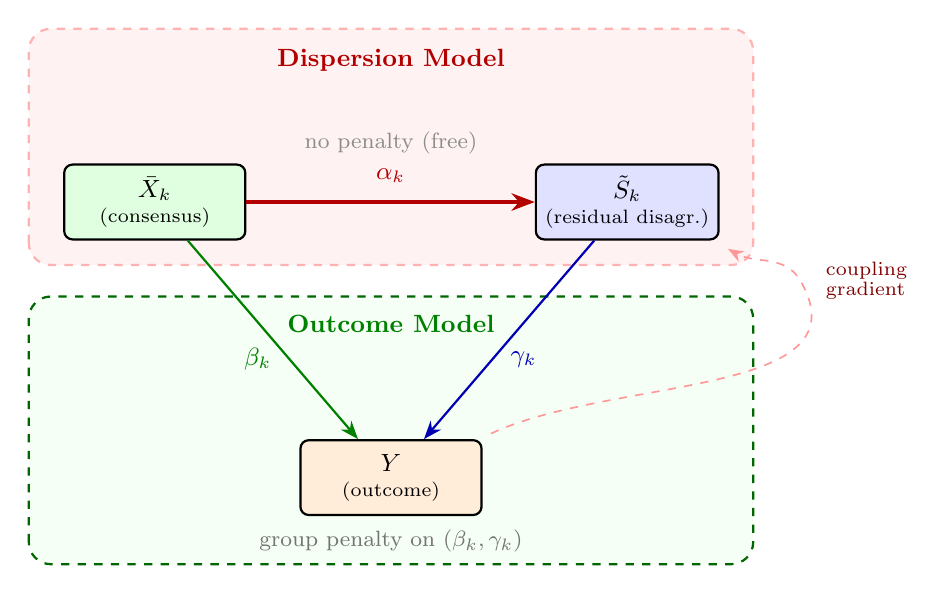
\begin{tikzpicture}[
  box/.style={rectangle, draw, rounded corners=3pt, minimum width=2.3cm, minimum height=0.95cm,
              align=center, font=\small, thick},
  arrow/.style={->, >=Stealth, thick},
]
  % Background regions
  \fill[red!5, rounded corners=8pt] (-4.6, -0.8) rectangle (4.6, 2.2);
  \draw[red!30, rounded corners=8pt, line width=0.8pt, dashed]
    (-4.6, -0.8) rectangle (4.6, 2.2);
  \fill[green!4, rounded corners=8pt] (-4.6, -4.6) rectangle (4.6, -1.2);
  \draw[green!40!black, rounded corners=8pt, line width=0.8pt, dashed]
    (-4.6, -4.6) rectangle (4.6, -1.2);

  % Nodes
  \node[box, fill=green!12] (X) at (-3.0, 0) {$\bar X_k$\\[-2pt]{\scriptsize(consensus)}};
  \node[box, fill=blue!12]  (S) at ( 3.0, 0) {$\tilde S_k$\\[-2pt]{\scriptsize(residual disagr.)}};
  \node[box, fill=orange!15](Y) at ( 0, -3.5) {$Y$\\[-2pt]{\scriptsize(outcome)}};

  % Dispersion model
  \node[font=\small\bfseries, text=red!70!black] at (0, 1.8) {Dispersion Model};
  \draw[arrow, red!70!black, very thick] (X) -- node[above=3pt, font=\small] {$\alpha_k$} (S);
  \node[font=\footnotesize, text=black!45] at (0, 0.75) {no penalty (free)};

  % Outcome model
  \node[font=\small\bfseries, text=green!50!black] at (0, -1.55) {Outcome Model};
  \draw[arrow, green!50!black] (X) -- node[left=3pt, font=\small, pos=0.6] {$\beta_k$} (Y);
  \draw[arrow, blue!70!black] (S) -- node[right=3pt, font=\small, pos=0.6] {$\gamma_k$} (Y);
  \node[font=\footnotesize, text=black!55] at (0, -4.3) {group penalty on $(\beta_k, \gamma_k)$};

  % Coupling gradient
  \draw[->, >=Stealth, red!40, dashed, line width=0.6pt]
    ([yshift=2pt, xshift=3pt]Y.north east) to[out=25, in=-60]
    (5.2, -1.0) to[out=120, in=-30]
    ([yshift=-3pt, xshift=3pt]S.south east);
  \node[font=\scriptsize, text=red!50!black, align=left, anchor=west] at (5.4, -1.0) {coupling\\[-1pt]gradient};
\end{tikzpicture}
\caption{Path diagram of the PRIMED model for feature $k$.
\textbf{Dispersion model (top):}
A linear regression links consensus $\bar X_k$ to disagreement via slope $\alpha_k$, estimated without penalty.
The residual disagreement $\tilde S_k$ captures the component of reader disagreement not explained by the consensus level.
\textbf{Outcome model (bottom):}
A logistic regression predicts $Y$ using consensus (via $\beta_k$) and residual disagreement (via $\gamma_k$), with a group penalty on $(\beta_k, \gamma_k)$.
Feature $k$ is selected when $(\hat\beta_k, \hat\gamma_k) \neq (0,0)$.
The dashed arrow indicates the coupling gradient: because $\tilde S_k$ depends on $\alpha_k$, the outcome loss feeds gradient updates to the dispersion parameters, achieving joint estimation.}\label{fig:path}
\end{figure}

%% --- Figure 2: Noise variable structure ---
\begin{figure}[h]
\centering
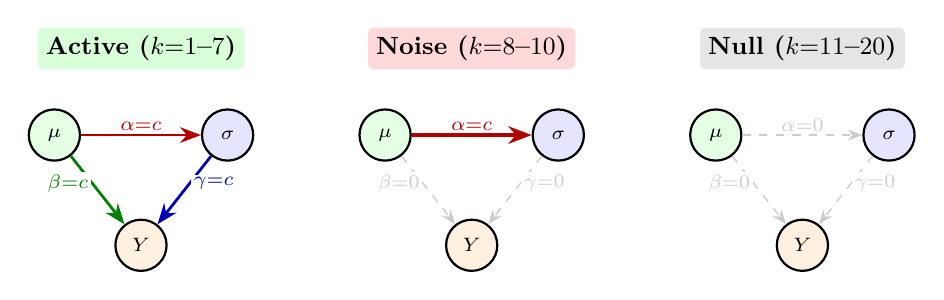
\begin{tikzpicture}[
  nd/.style={circle, draw, thick, minimum size=0.65cm, font=\scriptsize\bfseries},
  ar/.style={->, >=Stealth, thick},
  lb/.style={font=\scriptsize, fill=white, inner sep=1pt},
  grp/.style={font=\small\bfseries, rounded corners=2pt, inner sep=3pt}
]
\begin{scope}[shift={(0,0)}]
  \node[grp, fill=green!15] at (1.1, 2.3) {Active ($k{=}1$--$7$)};
  \node[nd, fill=green!10] (ma) at (0, 1.2) {$\mu$};
  \node[nd, fill=blue!10]  (sa) at (2.2, 1.2) {$\sigma$};
  \node[nd, fill=orange!12](ya) at (1.1, -0.2) {$Y$};
  \draw[ar, red!70!black, line width=1pt] (ma) -- node[lb, above] {$\alpha{=}c$} (sa);
  \draw[ar, green!50!black, line width=1pt] (ma) -- node[lb, left, pos=0.4] {$\beta{=}c$} (ya);
  \draw[ar, blue!70!black, line width=1pt] (sa) -- node[lb, right, pos=0.4] {$\gamma{=}c$} (ya);
\end{scope}
\begin{scope}[shift={(4.2,0)}]
  \node[grp, fill=red!15] at (1.1, 2.3) {Noise ($k{=}8$--$10$)};
  \node[nd, fill=green!10] (mn) at (0, 1.2) {$\mu$};
  \node[nd, fill=blue!10]  (sn) at (2.2, 1.2) {$\sigma$};
  \node[nd, fill=orange!12](yn) at (1.1, -0.2) {$Y$};
  \draw[ar, red!70!black, line width=1.2pt] (mn) -- node[lb, above] {$\alpha{=}c$} (sn);
  \draw[ar, gray!40, dashed, line width=0.5pt] (mn) -- node[lb, left, pos=0.4] {$\beta{=}0$} (yn);
  \draw[ar, gray!40, dashed, line width=0.5pt] (sn) -- node[lb, right, pos=0.4] {$\gamma{=}0$} (yn);
\end{scope}
\begin{scope}[shift={(8.4,0)}]
  \node[grp, fill=gray!20] at (1.1, 2.3) {Null ($k{=}11$--$20$)};
  \node[nd, fill=green!10] (mu) at (0, 1.2) {$\mu$};
  \node[nd, fill=blue!10]  (su) at (2.2, 1.2) {$\sigma$};
  \node[nd, fill=orange!12](yu) at (1.1, -0.2) {$Y$};
  \draw[ar, gray!40, dashed, line width=0.5pt] (mu) -- node[lb, above] {$\alpha{=}0$} (su);
  \draw[ar, gray!40, dashed, line width=0.5pt] (mu) -- node[lb, left, pos=0.4] {$\beta{=}0$} (yu);
  \draw[ar, gray!40, dashed, line width=0.5pt] (su) -- node[lb, right, pos=0.4] {$\gamma{=}0$} (yu);
\end{scope}
\end{tikzpicture}
\caption{Variable structure in the noise simulation.
Active variables (S2) have all three paths nonzero.
Noise variables have $\alpha \neq 0$ (reader disagreement present) but $\beta = \gamma = 0$ (no outcome relevance).
Null variables have no effect on any path.
In S1, noise variables are identical to null variables ($\alpha_{8\text{--}10} = 0$).}\label{fig:noise_structure}
\end{figure}

%% --- Figure 3: F1 vs tau (2x2 grid: DGP1/DGP2 x SNR) ---
\begin{figure}[h]
\centering
%% Row 1: DGP 1 (γ≠0), S2
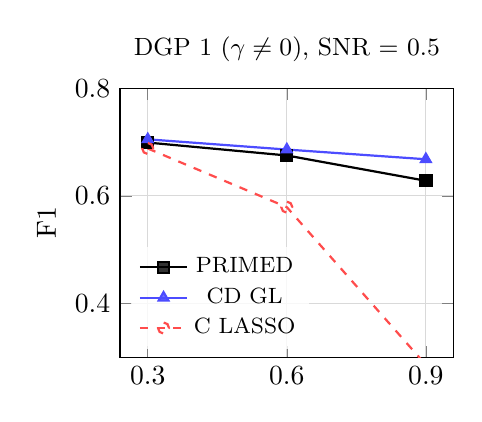
\begin{tikzpicture}
\begin{axis}[
  width=0.48\textwidth, height=5cm,
  xlabel={}, ylabel={F1},
  xtick={0.3,0.6,0.9}, ymin=0.3, ymax=0.8,
  legend style={at={(0.03,0.03)}, anchor=south west, font=\footnotesize, draw=none, fill=white, fill opacity=0.8, text opacity=1},
  title={\small DGP~1 ($\gamma \neq 0$), SNR = 0.5}, grid=major, grid style={gray!30},
  every axis plot/.append style={thick, mark size=2pt},
]
\addplot[color=black, mark=square*] coordinates {(0.3,0.699)(0.6,0.675)(0.9,0.628)};
\addplot[color=blue!70, mark=triangle*] coordinates {(0.3,0.705)(0.6,0.686)(0.9,0.668)};
\addplot[color=red!70, mark=o, dashed] coordinates {(0.3,0.688)(0.6,0.579)(0.9,0.286)};
\legend{PRIMED, CD GL, C LASSO}
\end{axis}
\end{tikzpicture}%
\hfill
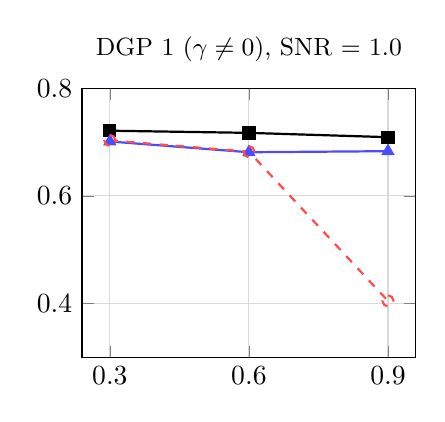
\begin{tikzpicture}
\begin{axis}[
  width=0.48\textwidth, height=5cm,
  xlabel={}, ylabel={},
  xtick={0.3,0.6,0.9}, ymin=0.3, ymax=0.8,
  title={\small DGP~1 ($\gamma \neq 0$), SNR = 1.0}, grid=major, grid style={gray!30},
  every axis plot/.append style={thick, mark size=2pt},
]
\addplot[color=black, mark=square*] coordinates {(0.3,0.721)(0.6,0.717)(0.9,0.709)};
\addplot[color=blue!70, mark=triangle*] coordinates {(0.3,0.701)(0.6,0.681)(0.9,0.683)};
\addplot[color=red!70, mark=o, dashed] coordinates {(0.3,0.703)(0.6,0.682)(0.9,0.405)};
\end{axis}
\end{tikzpicture}

\vspace{3pt}
%% Row 2: DGP 2 (γ=0), S2
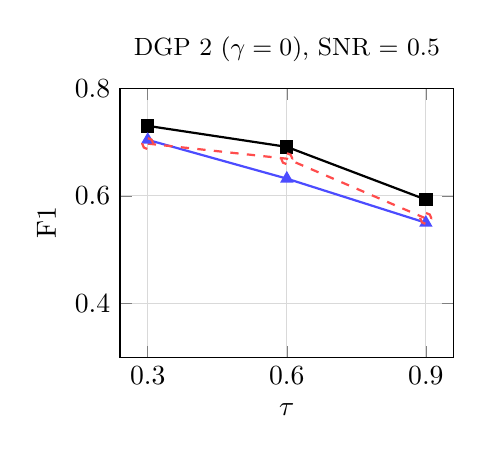
\begin{tikzpicture}
\begin{axis}[
  width=0.48\textwidth, height=5cm,
  xlabel={$\tau$}, ylabel={F1},
  xtick={0.3,0.6,0.9}, ymin=0.3, ymax=0.8,
  title={\small DGP~2 ($\gamma = 0$), SNR = 0.5}, grid=major, grid style={gray!30},
  every axis plot/.append style={thick, mark size=2pt},
]
\addplot[color=black, mark=square*] coordinates {(0.3,0.730)(0.6,0.691)(0.9,0.593)};
\addplot[color=blue!70, mark=triangle*] coordinates {(0.3,0.704)(0.6,0.632)(0.9,0.550)};
\addplot[color=red!70, mark=o, dashed] coordinates {(0.3,0.697)(0.6,0.669)(0.9,0.558)};
\end{axis}
\end{tikzpicture}%
\hfill
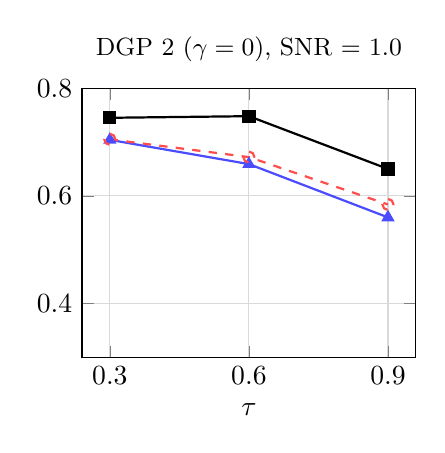
\begin{tikzpicture}
\begin{axis}[
  width=0.48\textwidth, height=5cm,
  xlabel={$\tau$}, ylabel={},
  xtick={0.3,0.6,0.9}, ymin=0.3, ymax=0.8,
  title={\small DGP~2 ($\gamma = 0$), SNR = 1.0}, grid=major, grid style={gray!30},
  every axis plot/.append style={thick, mark size=2pt},
]
\addplot[color=black, mark=square*] coordinates {(0.3,0.745)(0.6,0.748)(0.9,0.650)};
\addplot[color=blue!70, mark=triangle*] coordinates {(0.3,0.704)(0.6,0.659)(0.9,0.560)};
\addplot[color=red!70, mark=o, dashed] coordinates {(0.3,0.705)(0.6,0.672)(0.9,0.584)};
\end{axis}
\end{tikzpicture}
\caption{F1 score as a function of subject-specific noise $\tau$.
Results shown for S2 (noise present) under DGP~1 (top) and DGP~2 (bottom).
Under DGP~1, C~LASSO collapses at high $\tau$ because it ignores the disagreement channel that carries outcome signal.
Under DGP~2, C~LASSO remains stable since $\gamma = 0$, but PRIMED still achieves the highest F1 through superior PPV.}\label{fig:tau_f1}
\end{figure}

%% --- Figure 4: F1 vs K (2x2 grid: DGP1/DGP2 x SNR) ---
\begin{figure}[h]
\centering
%% Row 1: DGP 1 (γ≠0), S2
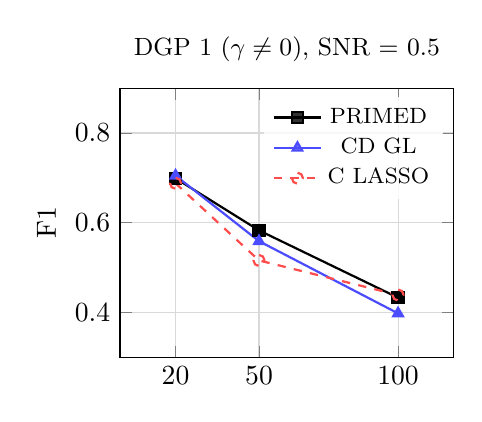
\begin{tikzpicture}
\begin{axis}[
  width=0.48\textwidth, height=5cm,
  xlabel={}, ylabel={F1},
  xtick={20,50,100}, xmin=0, xmax=120, ymin=0.3, ymax=0.9,
  legend style={at={(0.97,0.97)}, anchor=north east, font=\footnotesize, draw=none, fill=white, fill opacity=0.8, text opacity=1},
  title={\small DGP~1 ($\gamma \neq 0$), SNR = 0.5}, grid=major, grid style={gray!30},
  every axis plot/.append style={thick, mark size=2pt},
]
\addplot[color=black, mark=square*] coordinates {(20,0.699)(50,0.583)(100,0.433)};
\addplot[color=blue!70, mark=triangle*] coordinates {(20,0.705)(50,0.559)(100,0.398)};
\addplot[color=red!70, mark=o, dashed] coordinates {(20,0.688)(50,0.516)(100,0.439)};
\legend{PRIMED, CD GL, C LASSO}
\end{axis}
\end{tikzpicture}%
\hfill
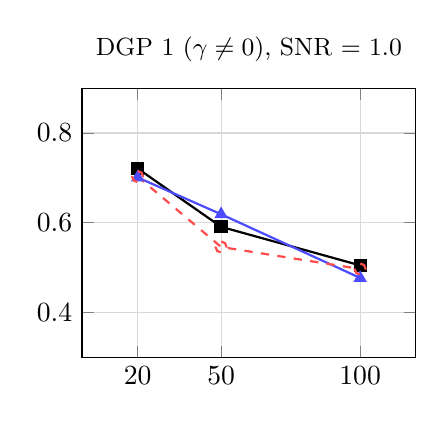
\begin{tikzpicture}
\begin{axis}[
  width=0.48\textwidth, height=5cm,
  xlabel={}, ylabel={},
  xtick={20,50,100}, xmin=0, xmax=120, ymin=0.3, ymax=0.9,
  title={\small DGP~1 ($\gamma \neq 0$), SNR = 1.0}, grid=major, grid style={gray!30},
  every axis plot/.append style={thick, mark size=2pt},
]
\addplot[color=black, mark=square*] coordinates {(20,0.721)(50,0.591)(100,0.505)};
\addplot[color=blue!70, mark=triangle*] coordinates {(20,0.701)(50,0.619)(100,0.477)};
\addplot[color=red!70, mark=o, dashed] coordinates {(20,0.703)(50,0.546)(100,0.497)};
\end{axis}
\end{tikzpicture}

\vspace{3pt}
%% Row 2: DGP 2 (γ=0), S2
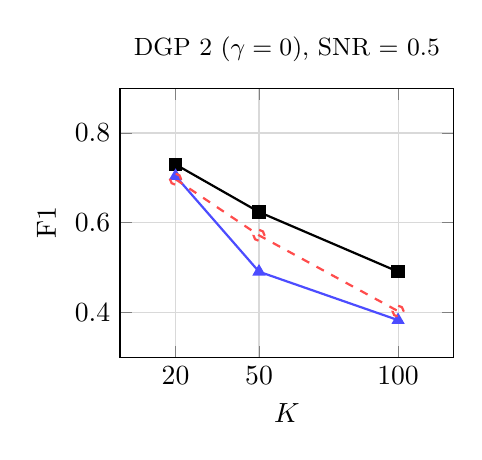
\begin{tikzpicture}
\begin{axis}[
  width=0.48\textwidth, height=5cm,
  xlabel={$K$}, ylabel={F1},
  xtick={20,50,100}, xmin=0, xmax=120, ymin=0.3, ymax=0.9,
  title={\small DGP~2 ($\gamma = 0$), SNR = 0.5}, grid=major, grid style={gray!30},
  every axis plot/.append style={thick, mark size=2pt},
]
\addplot[color=black, mark=square*] coordinates {(20,0.730)(50,0.624)(100,0.491)};
\addplot[color=blue!70, mark=triangle*] coordinates {(20,0.704)(50,0.491)(100,0.383)};
\addplot[color=red!70, mark=o, dashed] coordinates {(20,0.697)(50,0.572)(100,0.403)};
\end{axis}
\end{tikzpicture}%
\hfill
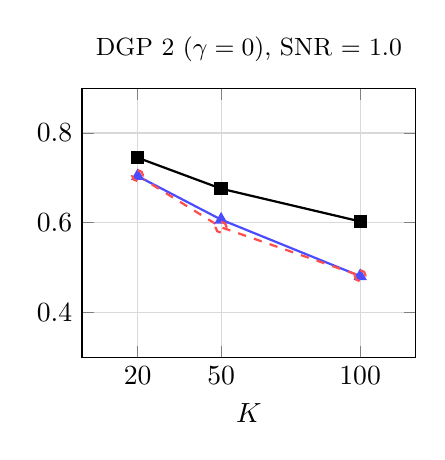
\begin{tikzpicture}
\begin{axis}[
  width=0.48\textwidth, height=5cm,
  xlabel={$K$}, ylabel={},
  xtick={20,50,100}, xmin=0, xmax=120, ymin=0.3, ymax=0.9,
  title={\small DGP~2 ($\gamma = 0$), SNR = 1.0}, grid=major, grid style={gray!30},
  every axis plot/.append style={thick, mark size=2pt},
]
\addplot[color=black, mark=square*] coordinates {(20,0.745)(50,0.676)(100,0.603)};
\addplot[color=blue!70, mark=triangle*] coordinates {(20,0.704)(50,0.607)(100,0.481)};
\addplot[color=red!70, mark=o, dashed] coordinates {(20,0.705)(50,0.590)(100,0.482)};
\end{axis}
\end{tikzpicture}
\caption{F1 score as a function of dimensionality $K$.
Results shown for S2 (noise present) under DGP~1 (top) and DGP~2 (bottom).
Under DGP~2, PRIMED maintains a consistent advantage (F1 gap $> .100$ at $K = 100$), driven by higher PPV when many inactive features have nontrivial dispersion structure.}\label{fig:dim_f1}
\end{figure}

%% --- Figure 5: Scatter plot ---
\begin{figure}[h]
\centering
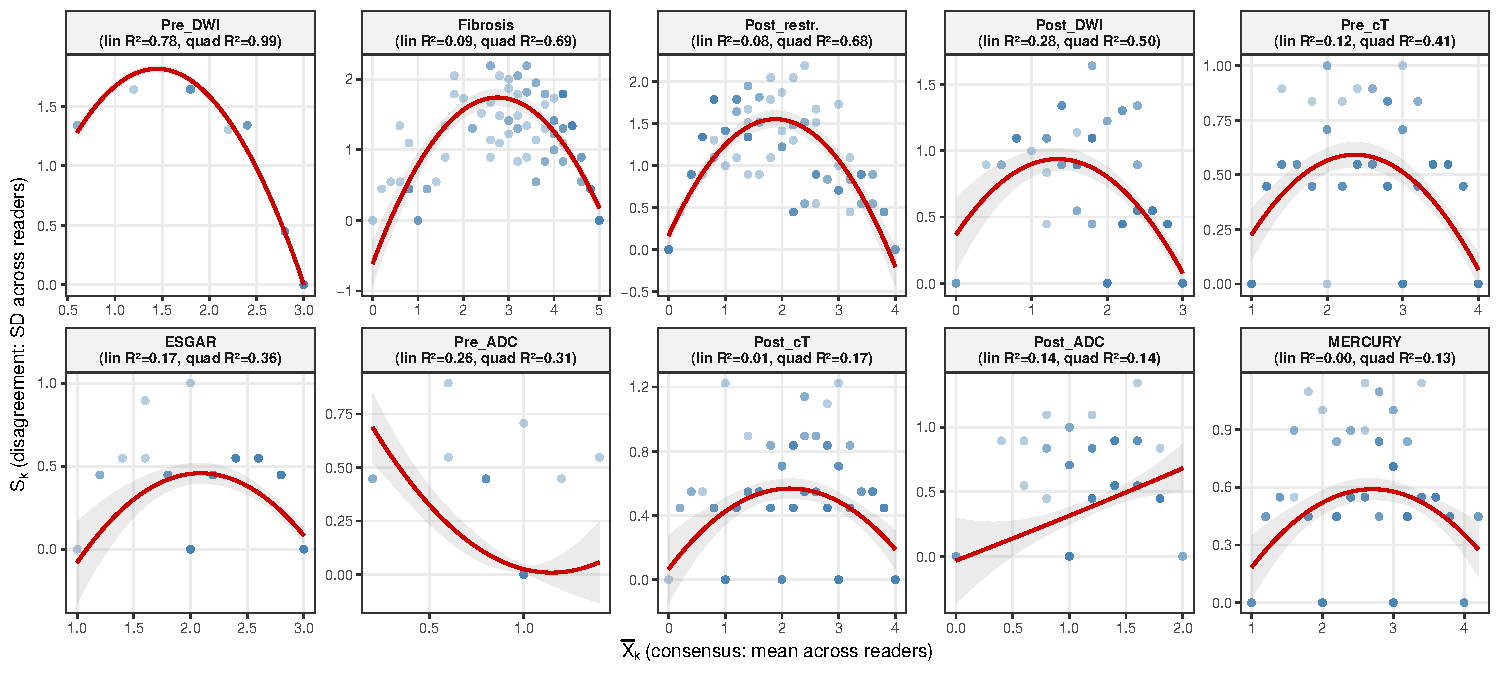
\includegraphics[width=\textwidth]{fig_scatter_cd.pdf}
\caption{Consensus--disagreement scatter plots for each ordinal feature.
The horizontal axis shows the consensus $\bar X_k$ (mean across five readers, $n = 149$) and the vertical axis shows the disagreement $S_k$ (standard deviation across readers).
Red curves indicate the fitted quadratic regression $S_k = \alpha_{0k} + \alpha_{1k} \bar X_k + \alpha_{2k} \bar X_k^2 + \varepsilon_k$; shaded bands show 95\% confidence intervals.
Panel titles report $R^2$ for both the linear and quadratic models.
Features are ordered by quadratic $R^2$; Pre\_DWI ($R^2 = 0.99$), Fibrosis ($R^2 = 0.69$), and Post\_restriction ($R^2 = 0.68$) show pronounced inverted-U patterns that the linear model fails to capture.}\label{fig:scatter_cd}
\end{figure}

%%===================================================================
%% Algorithm
%%===================================================================

\begin{algorithm}[h]
\caption{PRIMED: Proximal Gradient Descent with Selective Penalization}\label{alg:primed}
\begin{algorithmic}[1]
\Require $\bar X \in \mathbb{R}^{n \times K}$, $S \in \mathbb{R}^{n \times K}$, $Y \in \{0,1\}^n$, $\lambda > 0$, step size $\eta$, tolerance $\epsilon$, max iterations $T_{\max}$
\Ensure $\hat{\boldsymbol{\alpha}}, \hat{\boldsymbol{\beta}}, \hat{\boldsymbol{\gamma}}$
\Statex
\State \textbf{Initialize:} $\alpha_k \gets 0$, $\alpha_{0k} \gets \overline{S_k}$, $\beta_k \gets 0$, $\gamma_k \gets 0$, $\beta_0 \gets \mathrm{logit}(\bar Y)$
\State \textbf{Compute null losses:} $\mathcal{L}_{\mathrm{disp}}^0 \gets \tfrac{1}{2}\textstyle\sum_k \widehat{\mathrm{Var}}(S_k)$, \; $\mathcal{L}_{\mathrm{out}}^0 \gets -[\bar Y \log \bar Y + (1{-}\bar Y)\log(1{-}\bar Y)]$
\Statex
\For{$t = 1, 2, \dots, T_{\max}$}
  \Statex \quad \textit{\% Residual disagreement and predicted probabilities}
  \For{$k = 1, \dots, K$}
    \State $r_{ik} \gets S_{ik} - \alpha_{0k} - \alpha_k \bar X_{ik}$ \hfill \textit{\% $r_{ik} = \tilde S_{ik}$}
  \EndFor
  \For{$i = 1, \dots, n$}
    \State $p_i \gets \sigma(\beta_0 + \textstyle\sum_k \beta_k \bar X_{ik} + \gamma_k r_{ik})$
  \EndFor
  \Statex \quad \textit{\% Dispersion model gradients (normalized by $\mathcal{L}_{\mathrm{disp}}^0$)}
  \For{$k = 1, \dots, K$}
    \State $\alpha_{0k} \gets \alpha_{0k} + \eta \cdot \tfrac{1}{n \, \mathcal{L}_{\mathrm{disp}}^0} \textstyle\sum_i r_{ik}$
    \State $\alpha_k \gets \alpha_k + \eta \cdot \tfrac{1}{n \, \mathcal{L}_{\mathrm{disp}}^0} \textstyle\sum_i r_{ik} \bar X_{ik}$ \hfill \textit{\% dispersion gradient}
    \State $\alpha_k \gets \alpha_k + \eta \cdot \tfrac{\gamma_k}{n \, \mathcal{L}_{\mathrm{out}}^0} \textstyle\sum_i (p_i - Y_i) \bar X_{ik}$ \hfill \textit{\% coupling gradient}
    \State $\alpha_{0k} \gets \alpha_{0k} + \eta \cdot \tfrac{\gamma_k}{n \, \mathcal{L}_{\mathrm{out}}^0} \textstyle\sum_i (p_i - Y_i)$ \hfill \textit{\% intercept coupling}
  \EndFor
  \Statex \quad \textit{\% Outcome model gradients (normalized by $\mathcal{L}_{\mathrm{out}}^0$)}
  \State $\beta_0 \gets \beta_0 - \eta \cdot \tfrac{1}{n \, \mathcal{L}_{\mathrm{out}}^0} \textstyle\sum_i (p_i - Y_i)$
  \For{$k = 1, \dots, K$}
    \State $\tilde\beta_k \gets \beta_k - \eta \cdot \tfrac{1}{n \, \mathcal{L}_{\mathrm{out}}^0} \textstyle\sum_i (p_i - Y_i)\bar X_{ik}$
    \State $\tilde\gamma_k \gets \gamma_k - \eta \cdot \tfrac{1}{n \, \mathcal{L}_{\mathrm{out}}^0} \textstyle\sum_i (p_i - Y_i) r_{ik}$
  \EndFor
  \Statex \quad \textit{\% Proximal step: group soft-thresholding on $(\beta_k, \gamma_k)$}
  \For{$k = 1, \dots, K$}
    \If{$\|(\tilde\beta_k, \tilde\gamma_k)\|_2 > \eta\lambda\sqrt{2}$}
      \State $(\beta_k, \gamma_k) \gets \bigl(1 - \tfrac{\eta\lambda\sqrt{2}}{\|(\tilde\beta_k, \tilde\gamma_k)\|_2}\bigr)(\tilde\beta_k, \tilde\gamma_k)$
    \Else
      \State $(\beta_k, \gamma_k) \gets (0, 0)$
    \EndIf
  \EndFor
  \Statex \quad \textit{\% Convergence check}
  \If{relative change in parameters $< \epsilon$}
    \State \textbf{break}
  \EndIf
\EndFor
\Statex
\State \textbf{Selection:} feature $k$ is selected if $\hat\beta_k \neq 0$ or $\hat\gamma_k \neq 0$
\end{algorithmic}
\end{algorithm}


%%===================================================================
\backmatter
%%===================================================================

\bmhead{List of abbreviations}

\noindent
pCR: pathologic complete response;
CRT: chemoradiation therapy;
MRI: magnetic resonance imaging;
CD: consensus--disagreement;
PRIMED: Penalized Regularization for Integrated Multi-path Estimation with Dispersion;
GL: group LASSO;
C~LASSO: consensus LASSO;
OLS: ordinary least squares;
DGP: data generating process;
SNR: signal-to-noise ratio;
TPR: true positive rate;
PPV: positive predictive value;
AUC: area under the receiver operating characteristic curve;
DWI: diffusion-weighted imaging;
ADC: apparent diffusion coefficient;
ESGAR: European Society of Gastrointestinal and Abdominal Radiology;
ICC: intraclass correlation coefficient;
SD: standard deviation;
LIDC-IDRI: Lung Image Database Consortium and Image Database Resource Initiative;
HU: Hounsfield units;
CT: computed tomography;
CV: cross-validation;


\section*{Declarations}

\subsection*{Ethics approval and consent to participate}
This study was approved by the institutional review board of each participating center. Informed consent was obtained from all participants. The LIDC-IDRI dataset is publicly available and does not require separate ethics approval.

\subsection*{Consent for publication}
Not applicable.

\subsection*{Availability of data and materials}
The LIDC-IDRI dataset analysed during the current study is publicly available in The Cancer Imaging Archive (TCIA) repository \cite{TCIA2015}. The rectal cancer MRI dataset used during the current study is available from the corresponding author on reasonable request. All analysis code, including the PRIMED implementation, simulation scripts, and application code, is publicly available at \texttt{https://github.com/yonghankwon0/PRIMED}.

\subsection*{Competing interests}
The authors declare that they have no competing interests.

\subsection*{Funding}
Not applicable.

\subsection*{Authors' contributions}
YK conceived the study, developed the methodology, implemented the algorithms, performed all analyses, and drafted the manuscript. KH supervised the study and critically revised the manuscript. All authors read and approved the final manuscript.

\subsection*{Acknowledgements}
Not applicable.


%%===================================================================
\begin{appendices}
%%===================================================================

\section{Consensus--disagreement measures for multi-reader data}\label{secA1}

PRIMED requires two subject-level summaries per feature: a consensus measure and a disagreement (dispersion) measure.
In Section~\ref{sec:methods} we use the sample mean and sample standard deviation, which are the natural choices when features are continuous or ordinal with five or more categories.
This appendix catalogues alternatives for different measurement scales, so that PRIMED can be applied to a broader range of multi-reader data.
The two applications in this paper illustrate different ends of this spectrum: the rectal cancer study (Section~\ref{sec:application}) uses ordinal MRI features scored on 3--6 point scales (10 ordinal plus 4 binary features, $K = 14$ total, $m = 5$ readers), while the LIDC-IDRI study (Section~\ref{sec:lidc}) uses continuous radiomics features extracted from 3D segmentation masks ($K = 107$, $m = 3$--$4$ readers).

Throughout, $R$ readers evaluate a subject on a single feature, producing scores $X_1, \dots, X_R$.

\subsection{Guiding principles}\label{secA1:principles}

\paragraph{Subject-level measures are required.}
Global agreement indices such as ICC \cite{Shrout1979} and Fleiss' $\kappa$ \cite{Fleiss1971} produce a single number for the entire dataset.
PRIMED, by contrast, needs one consensus value and one disagreement value \emph{per subject per feature}, so that each patient's degree of reader disagreement can enter the model as a predictor.

\paragraph{When disagreement is informative.}
The dispersion model $S_k = \alpha_{0k} + \alpha_k \bar X_k + \varepsilon_k$ is most useful when $\alpha_k \neq 0$, i.e., when disagreement depends systematically on the consensus level.
Common patterns include negative linear (disagreement decreases near the scale boundaries), positive linear, and inverted-U-shaped (disagreement peaks at intermediate scores).
When nonlinear patterns are present, the quadratic extension $S_k = \alpha_{0k} + \alpha_{1k} \bar X_k + \alpha_{2k} \bar X_k^2 + \varepsilon_k$ (Section~\ref{sec:nonlinear}) can substantially improve the explained variance; e.g., from $R^2 = 0.085$ to $0.695$ for Fibrosis in the rectal cancer data (Table~\ref{tab:disp_r2}).
In the LIDC-IDRI radiomics data, 77 of 107 features show higher quadratic than linear $R^2$.
If $S_k$ is approximately constant across subjects, the dispersion channel adds little information.

\subsection{Continuous features}\label{secA2}

For continuous features, the arithmetic mean and standard deviation are the default consensus and disagreement measures used in PRIMED (Section~\ref{sec:methods}).
This is the setting used in the LIDC-IDRI radiomics application (Section~\ref{sec:lidc}), where each feature is a continuous quantity (e.g., volume in mm$^3$, entropy in nats) computed independently from each reader's segmentation mask.
When features span very different scales, standardization prior to model fitting is recommended; in our implementation, both $\bar X_k$ and $S_k$ are centered and scaled to unit variance within the training set.
Table~\ref{tab:continuous_measures} lists alternatives.

\begin{table}[h]
\caption{Consensus and dispersion measures for continuous features}\label{tab:continuous_measures}
\small
\renewcommand{\arraystretch}{1.3}
\begin{tabular*}{\textwidth}{@{\extracolsep\fill}l l p{0.32\textwidth} l}
\toprule
Type & Measure & Formula & Properties \\
\midrule
\multirow{3}{*}{Consensus}
& Arithmetic mean & $\bar X = R^{-1}\sum_{r=1}^R X_r$ & Default in PRIMED \\
& Median & $\mathrm{Med}(X_1,\dots,X_R)$ & Robust to outliers \\
& Trimmed mean & Mean after removing top/bottom $k$\% & Compromise \\
\midrule
\multirow{4}{*}{Dispersion}
& SD & $\bigl[\frac{1}{R-1}\sum_{r=1}^R(X_r-\bar X)^2\bigr]^{1/2}$ & Default in PRIMED \\
& Range & $\max_r X_r - \min_r X_r$ & Simple \\
& Mean abs.\ deviation & $R^{-1}\sum_{r=1}^R |X_r - \bar X|$ & Robust to outliers \\
& Coeff.\ of variation & $\mathrm{SD}/\bar X$ & Scale-invariant \\
\botrule
\end{tabular*}
\end{table}

\subsection{Ordinal features}\label{secA3}

For ordinal scales with five or more categories, treating the data as approximately continuous and using the mean and SD is well supported \cite{Norman2010,Sullivan2013}.
In the rectal cancer application (Section~\ref{sec:application}), all 10 ordinal MRI features (scored on 3--6 point scales by five radiologists) are summarized using the mean and SD, following this continuous approximation.
For shorter scales (3--4 categories), ordinal-specific dispersion measures may be preferred as alternatives.

\paragraph{Within-group agreement ($r_{WG}$).}
The $r_{WG}$ index \cite{James1984} compares the observed variance $S_X^2$ to the expected variance $\sigma_E^2$ under random responding:
$r_{WG} = 1 - S_X^2 / \sigma_E^2$.
Under a uniform null on $A$ response options, $\sigma_E^2 = (A^2-1)/12$.

\paragraph{Average deviation ($AD_M$).}
The average deviation around the mean \cite{Burke1999},
$AD_M = R^{-1}\sum_{r=1}^R |X_r - \bar X|$,
is more robust to outliers than SD. Agreement is judged adequate when $AD_M < c/6$, where $c$ is the number of response options.

\paragraph{Leik's ordinal dispersion ($D$).}
Leik's $D$ \cite{Leik1966} uses the cumulative frequency distribution: $D = 0$ indicates perfect consensus and $D = 1$ indicates maximum dispersion.

\paragraph{Ordinal variation ($1 - l^2$).}
Blair and Lacy's ordinal variation \cite{Blair2000} measures how far the cumulative distribution lies from a maximum-dispersion configuration, ranging from 0 (perfect consensus) to 1 (maximum dispersion).

Table~\ref{tab:ordinal_summary} summarizes the available measures by scale length. Both applications in this paper use the mean and SD for all ordinal features.

\begin{table}[h]
\caption{Available consensus and dispersion measures for ordinal features}\label{tab:ordinal_summary}
\small
\renewcommand{\arraystretch}{1.2}
\begin{tabular*}{\textwidth}{@{\extracolsep\fill}ll l p{0.33\textwidth}}
\toprule
Scale & Consensus & Dispersion & Rationale \\
\midrule
5+ categories & Mean & SD, $r_{WG}$, $AD_M$ & Treat as continuous \\
3--4 categories & Mean or Median & SD, Leik's $D$, $1-l^2$ & Mean/SD used in this paper; ordinal-specific alternatives available \\
\botrule
\end{tabular*}
\end{table}

\subsection{Binary features}\label{secA4}

For binary features ($X_r \in \{0,1\}$), the standard deviation $\sqrt{p(1-p)}$ is a deterministic function of the consensus proportion $p = \bar X$.
Including both as predictors would introduce perfect multicollinearity.
PRIMED therefore uses \emph{only the consensus mean} for binary features, applying a LASSO penalty rather than the group penalty used for ordinal features.
This is the approach taken in the rectal cancer application (Section~\ref{sec:application}), where four binary MRI features enter the model as reader-averaged proportions.
The LIDC-IDRI application does not involve binary features, as all 107 radiomics features are continuous.

\subsection{Nominal features}\label{secA5}

For nominal features with $C \geq 3$ unordered categories, let $p_c$ denote the proportion of readers selecting category $c$.
Unlike binary features, nominal features admit nontrivial dispersion measures.
Table~\ref{tab:nominal_measures} lists the most common options.

\begin{table}[h]
\caption{Consensus and dispersion measures for nominal features ($C \geq 3$ categories)}\label{tab:nominal_measures}
\small
\renewcommand{\arraystretch}{1.3}
\begin{tabular*}{\textwidth}{@{\extracolsep\fill}lll}
\toprule
Measure & Formula & Range \\
\midrule
Mode (consensus) & $\arg\max_c\, p_c$ & --- \\
Agreement rate & $\max_c\, p_c$ & $[1/C,\; 1]$ \\
Simpson's diversity & $1 - \sum_{c=1}^C p_c^2$ & $[0,\; 1-1/C]$ \\
Shannon entropy & $-\sum_{c=1}^C p_c \log_2 p_c$ & $[0,\; \log_2 C]$ \\
\botrule
\end{tabular*}
\end{table}

\subsection{Summary}\label{secA6}

Table~\ref{tab:scale_summary} summarizes how PRIMED handles each measurement scale.

\begin{table}[h]
\caption{Summary of consensus and dispersion measures by measurement scale}\label{tab:scale_summary}
\footnotesize
\renewcommand{\arraystretch}{1.3}
\begin{tabular*}{\textwidth}{@{\extracolsep\fill}lll p{0.18\textwidth} l}
\toprule
Scale & Consensus & Dispersion & PRIMED penalty & Application \\
\midrule
Continuous & Mean & SD & Group $(\beta_k, \gamma_k)$ & LIDC-IDRI \\
Ordinal & Mean & SD & Group $(\beta_k, \gamma_k)$ & Rectal \\
Binary & Mean ($= p$) & N/A & LASSO ($\delta_k$) & Rectal \\
Nominal ($\geq$3 cat.) & Mode & Entropy / Simpson's $D$ & Group $(\beta_k, \gamma_k)$ & --- \\
\botrule
\end{tabular*}
\end{table}

\section{Data-driven regularization path}\label{secA_lambda}

The regularization parameter $\lambda$ controls the sparsity of the PRIMED solution.
We construct a data-driven path following the approach of Friedman et al.\ \cite{Friedman2010}.

\subsection{Computing $\lambda_{\max}$}

At the null model ($\beta_k = \gamma_k = 0$ for all $k$), the predicted probability is $\hat p_i = \bar Y$ for all $i$, and the residual disagreement reduces to $\tilde S_{ik} = S_{ik} - \bar S_k$.
The gradient of the outcome loss with respect to $(\beta_k, \gamma_k)$ is
\[
  g_k = \Bigl(\frac{1}{n\,\mathcal{L}_{\mathrm{out}}^0}\sum_i (\bar Y - Y_i)\bar X_{ik},\;\;
        \frac{1}{n\,\mathcal{L}_{\mathrm{out}}^0}\sum_i (\bar Y - Y_i)(S_{ik} - \bar S_k)\Bigr).
\]
The proximal step sets $(\beta_k, \gamma_k) = (0,0)$ whenever $\|g_k\|_2 \leq \eta\lambda\sqrt{2}$.
Therefore, all features are deselected when
\[
  \lambda \geq \lambda_{\max} \;=\; \frac{1}{\sqrt{2}}\max_{k=1,\dots,K} \|g_k\|_2.
\]

\subsection{Log-spaced grid}

Given $\lambda_{\max}$, we construct a grid of $L$ values log-spaced on $[\lambda_{\max} \cdot \epsilon,\; \lambda_{\max}]$, where $\epsilon = 0.01$ (simulations, $K \leq 100$) or $\epsilon = 0.001$ (LIDC-IDRI application, $K = 107$, where the larger feature space benefits from finer resolution at small $\lambda$):
\[
  \lambda_j = \lambda_{\max} \cdot \exp\!\Bigl(\frac{j-1}{L-1} \log \epsilon\Bigr), \quad j = 1,\dots,L.
\]
This ensures dense coverage near $\lambda_{\max}$ (where the transition from null to non-null models occurs) and sparser coverage at small $\lambda$ values.


\section{Rectal cancer MRI feature descriptions}\label{app:rectal_features}

Table~\ref{tab:rectal_features} lists all $K = 14$ MRI features used in the rectal cancer application (Section~\ref{sec:application}).
Ten ordinal features are scored on 3--6 point scales by five radiologists; their consensus and disagreement are computed as the sample mean and standard deviation, respectively.
Four binary features are scored as present or absent; their consensus enters the model as the reader-averaged proportion (Appendix~\ref{secA4}).

\begin{table}[h]
\caption{MRI features in the rectal cancer application}\label{tab:rectal_features}
\footnotesize
\renewcommand{\arraystretch}{1.1}
\begin{tabular*}{\textwidth}{@{\extracolsep\fill}llc}
\toprule
Feature & Scale & Categories \\
\midrule
\multicolumn{3}{l}{\textit{Ordinal features (consensus = mean, disagreement = SD)}} \\[2pt]
Fibrosis grading & Normalized wall to viable tumor & 6 \\
Pre\_cT & T stage (partial to T3c+/T4) & 4 \\
Pre\_DWI & DWI signal (not seen / low / iso / high) & 4 \\
Pre\_ADC & ADC signal (not seen / low / iso / high) & 4 \\
Post\_cT & T stage (normalized to T3c+) & 5 \\
Post\_DWI & DWI signal (not seen / low / iso / high) & 4 \\
Post\_ADC & ADC signal (not seen / low / iso / high) & 4 \\
Post\_restriction & Restriction (none to diffuse) & 5 \\
MERCURY & Tumor regression grade (1--5) & 5 \\
ESGAR & Normal / fibrosis only / residual tumor & 3 \\
\midrule
\multicolumn{3}{l}{\textit{Binary features (consensus = proportion, no disagreement channel)}} \\[2pt]
Split scar & Absent / present & 2 \\
Ulcer & Absent / present & 2 \\
Pre\_EMVI & Absent / present & 2 \\
Normalized wall & Absent / present & 2 \\
\botrule
\end{tabular*}
\footnotetext{DWI: diffusion-weighted imaging; ADC: apparent diffusion coefficient; EMVI: extramural vascular invasion; ESGAR: European Society of Gastrointestinal and Abdominal Radiology; MERCURY: Magnetic Resonance Imaging and Rectal Cancer European Equivalence Study.}
\end{table}

\section{LIDC-IDRI preprocessing details}\label{secA_lidc}

\subsection{CT windowing}

CT images contain Hounsfield unit (HU) values spanning a wide range: air appears at approximately $-1000$~HU, soft tissue at $-100$ to $+100$~HU, and cortical bone above $+400$~HU.
Because lung nodules are soft-tissue structures, voxels near the mask boundary may include air (lung parenchyma) or bone (ribs, vertebrae) that are not part of the nodule itself.
When different readers draw slightly different contours, these boundary voxels are included in some masks but not others, inflating the measured reader disagreement with artifact rather than genuine diagnostic uncertainty.

We apply CT windowing by clipping all voxel values to $[-1000, 400]$~HU before feature extraction:
\[
  v_i \gets \max(-1000, \min(400, v_i)).
\]
This removes extreme values from air and bone while preserving the full dynamic range of soft tissue.

\subsection{PyRadiomics feature classes}

The 107 radiomics features extracted per reader per nodule comprise seven classes from the PyRadiomics library \cite{vanGriethuysen2017}:
Shape (14 features: volume, surface area, sphericity, elongation, etc.),
First-order (18: mean, variance, entropy, skewness, kurtosis, energy, etc.),
GLCM (24: contrast, correlation, homogeneity, energy, etc.),
GLRLM (16: short/long run emphasis, gray level non-uniformity, etc.),
GLSZM (16: small/large area emphasis, zone entropy, etc.),
NGTDM (5: coarseness, busyness, complexity, strength, contrast),
and GLDM (14: dependence variance, entropy, etc.).
All features are extracted with bin width 25, $1 \times 1 \times 1$~mm isotropic resampling, and B-spline interpolation.

\end{appendices}

%%===================================================================
%% References
%%===================================================================
\bibliography{sn-bibliography}

\end{document}
